\subsection{\ystar\ cut Optimization}
\label{section:ystarCutOptimization}

%\todo[inline]{ Clean up formulae. }

In QCD two-to-two scattering, $t$-channel is dominant. The QCD dijet production is proportional to 
$\displaystyle{(1-\cos\theta^{*})^{-2}}$, while $H^\prime$ and String production is expected to be flat in 
$\cos\theta^{*}$. This means that \ystar\  of QCD background will minimize at 0 and that of $H^\prime$  
and String will peak at 0.


The significance is given by 
\begin{equation}
%\label{eq:signifcanceYstar} % uncomment if label used.
S  = \sqrt{\sum_{i}{2\left[ \left(S_{i}+B_{i} \right)\cdot \ln \left(1+\frac{S_{i}}{B_{i}}\right)-S_{i}\right]}}
\end{equation}
where $S_i$ ($B_i$) is the number of signal (background) events in bin $i$. 
Figure \ref{fig: hprime significance as a function of y* cut} shows $H^\prime$ signal significance as a function 
of the value of the \ystar\  cut. The significance peaks  around 0.6, so the optimal $y^{*}$ cut for the $H'$ search is 
$|\ystar| < 0.6$. Figure \ref{fig: string significance as a function of y* cut} shows the String signal significance as a function of \ystar\ cut. The significance peaks at  0.8, so the optimal  cut for the String search is $|\ystar| < 0.8$.

\begin{figure}[htbp]
        \centering
        \subfigure[$\geq$1 g-tag]{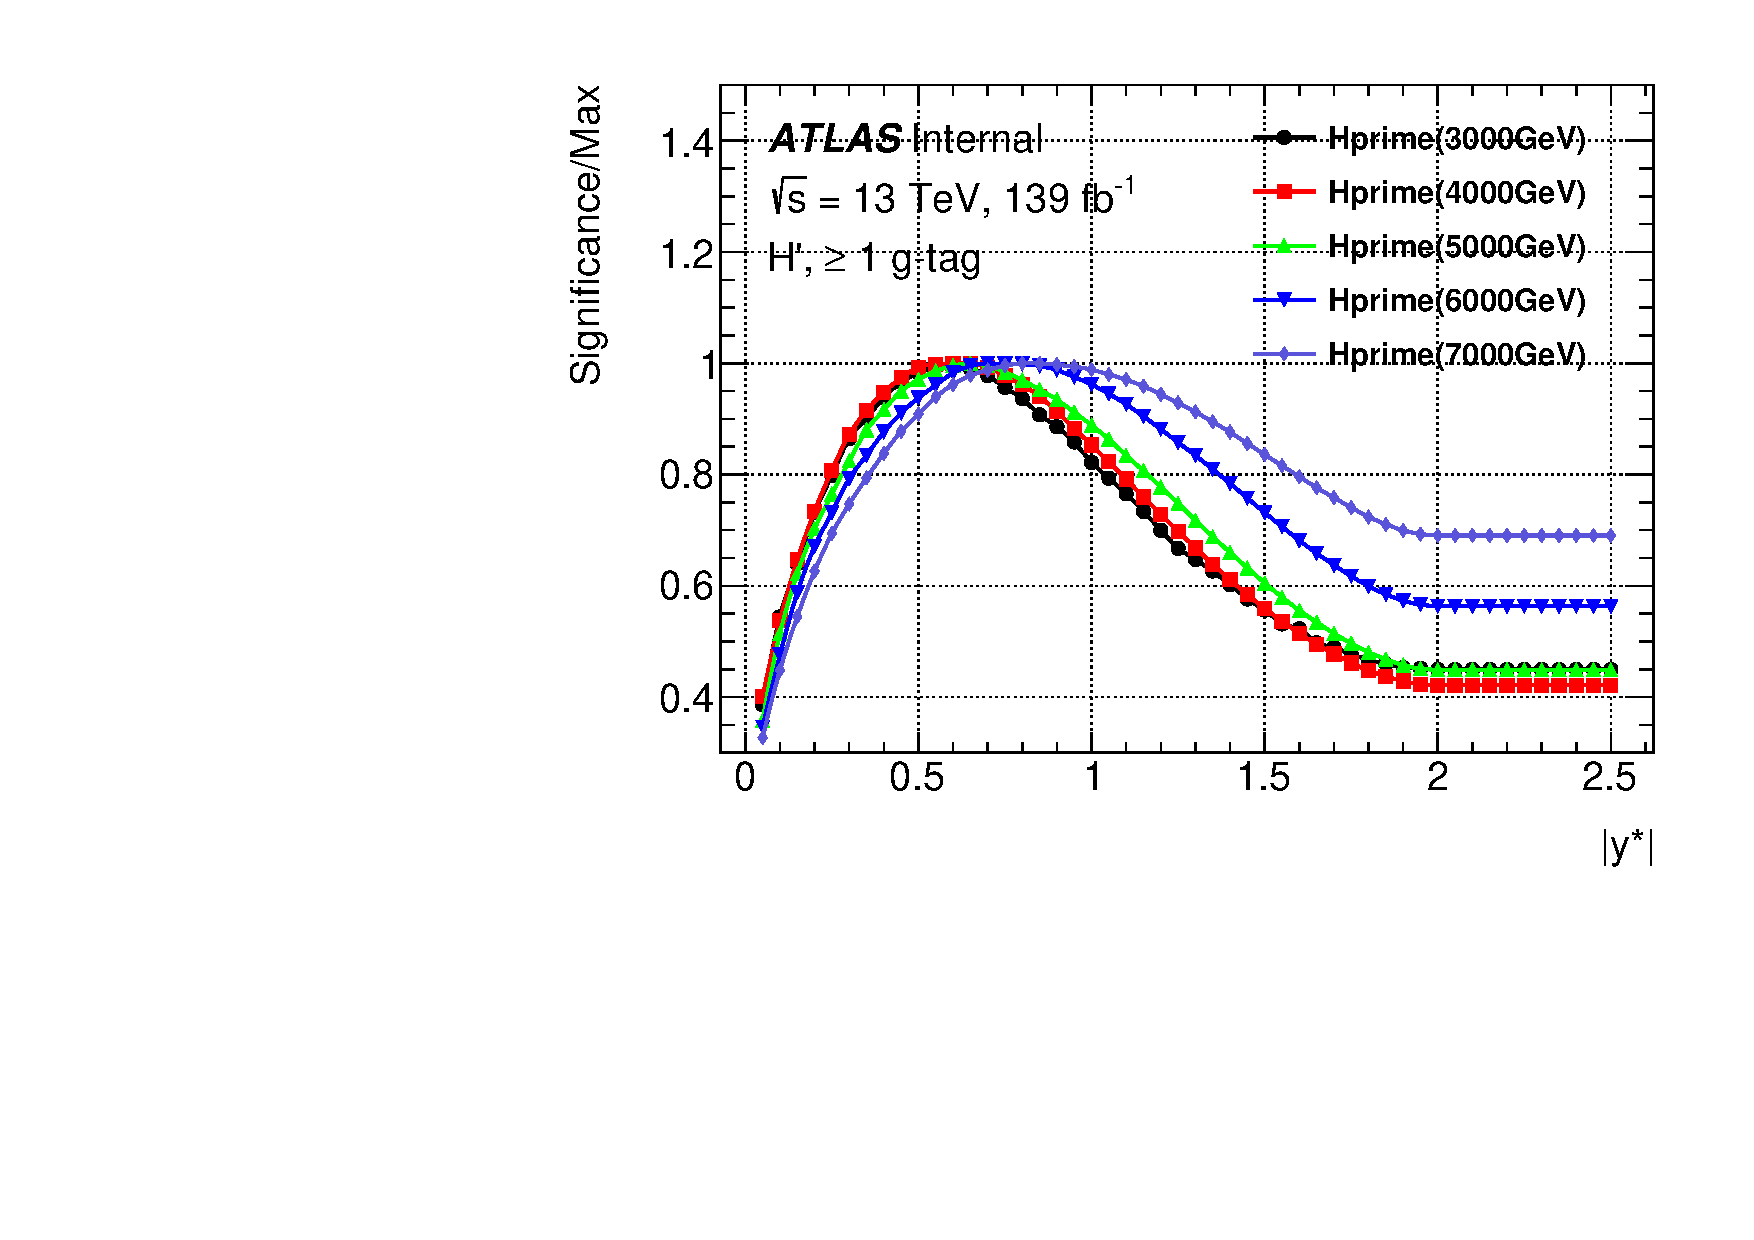
\includegraphics[width=0.48\columnwidth]{figures/yStarOptimization/Significance_Hprime_gj.pdf}}
        \subfigure[2 g-tag]{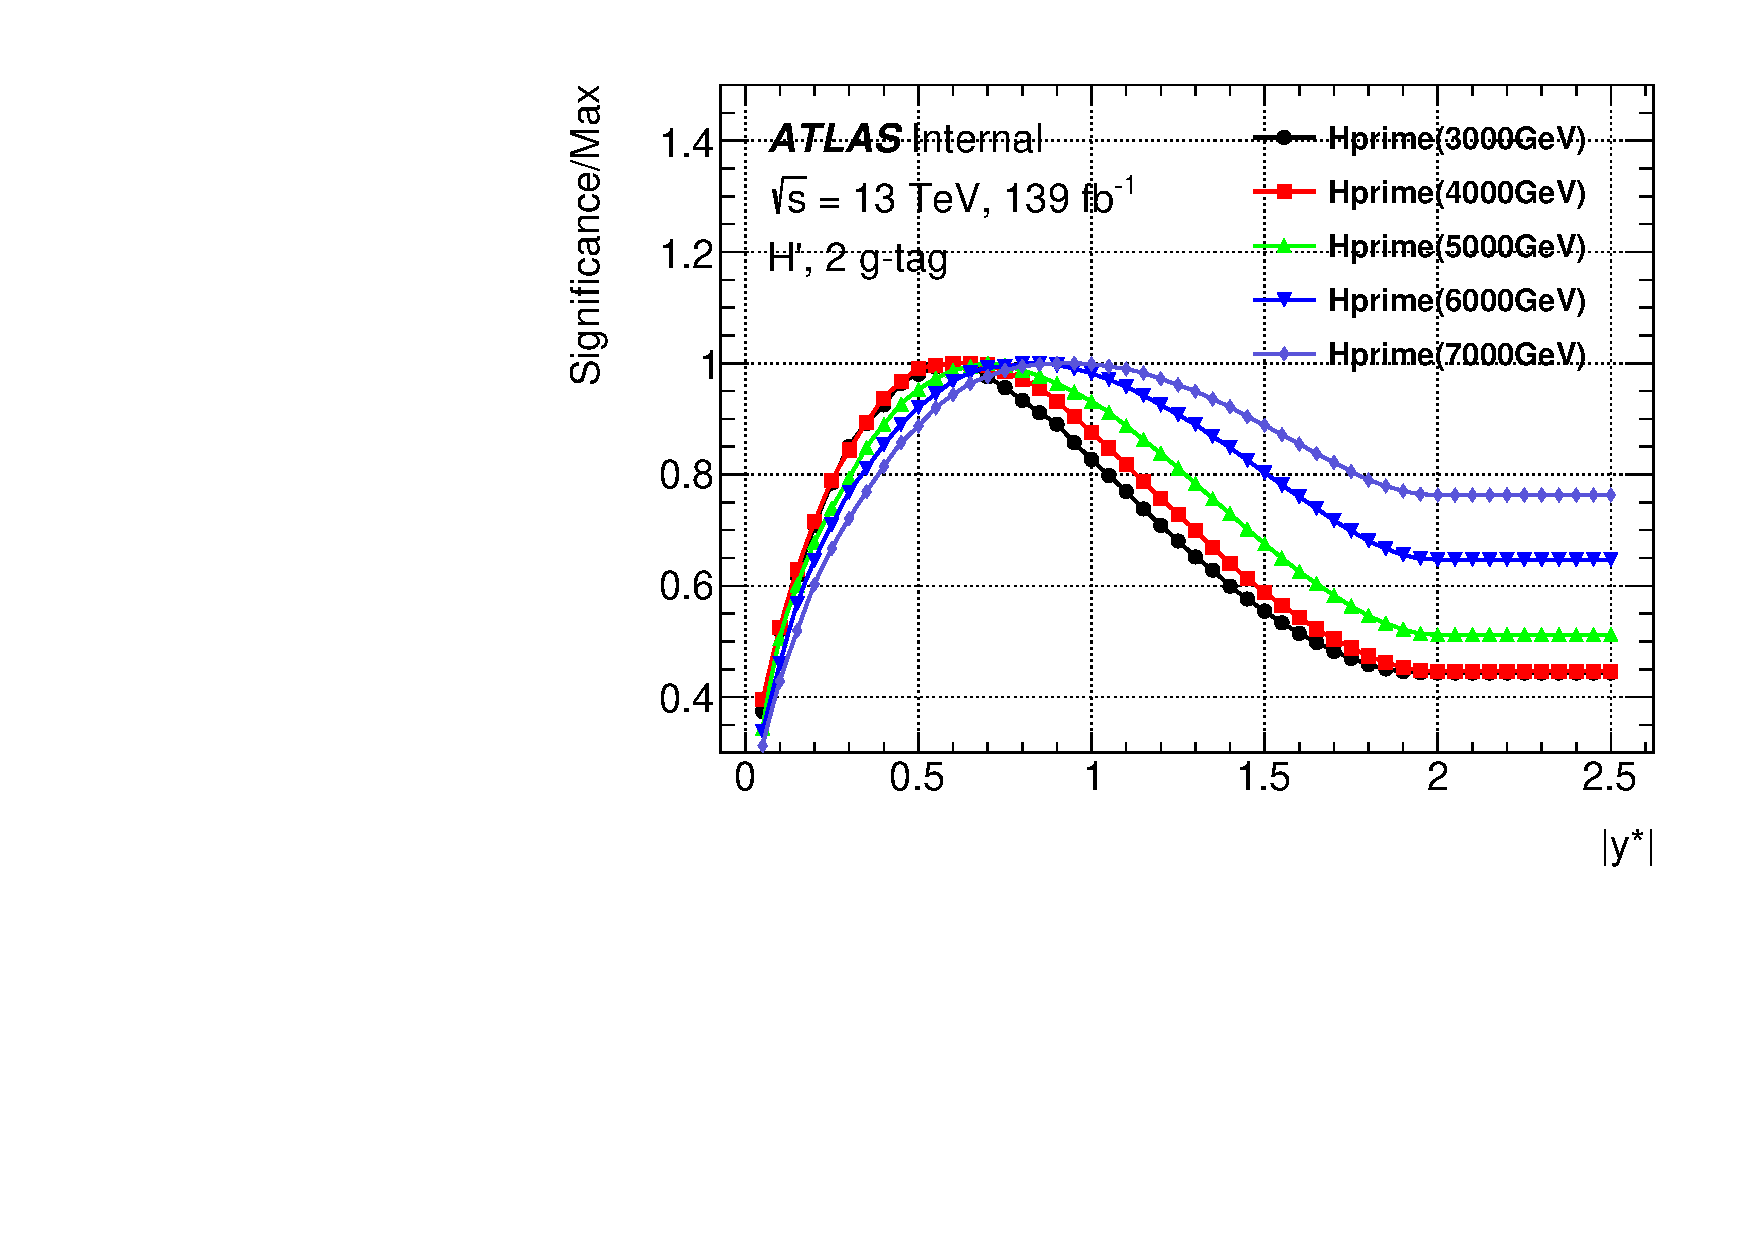
\includegraphics[width=0.48\columnwidth]{figures/yStarOptimization/Significance_Hprime_gg.pdf}}
        \caption{$H^\prime$ significance as a function \ystar\ cut in the case of (a) $\geq$1 g-tag, (b) 2 g-tag.}
        \label{fig: hprime significance as a function of y* cut}
\end{figure}


\begin{figure}[htbp]
        \centering
        \subfigure[$\geq$1 g-tag]{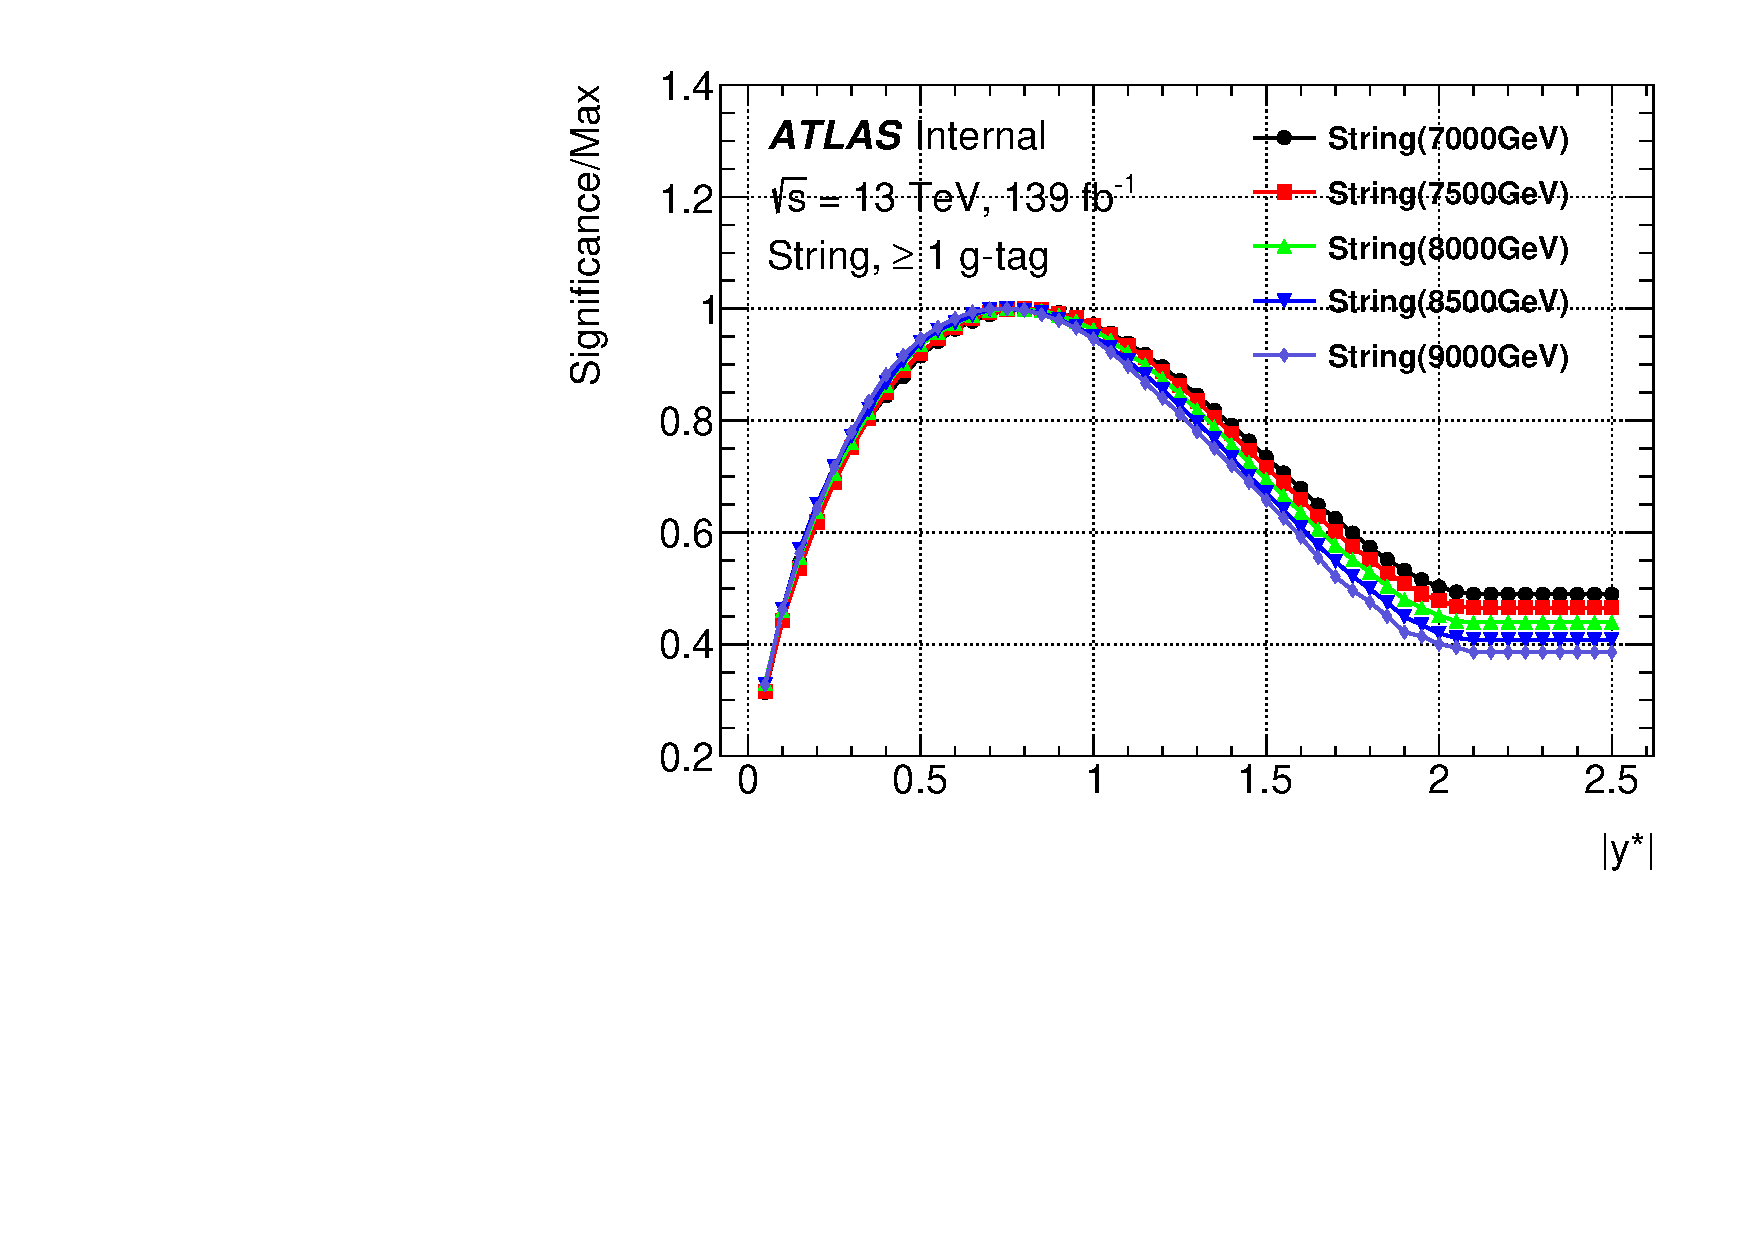
\includegraphics[width=0.48\columnwidth]{figures/yStarOptimization/Significance_String_gj.pdf}}
        \subfigure[2 g-tag]{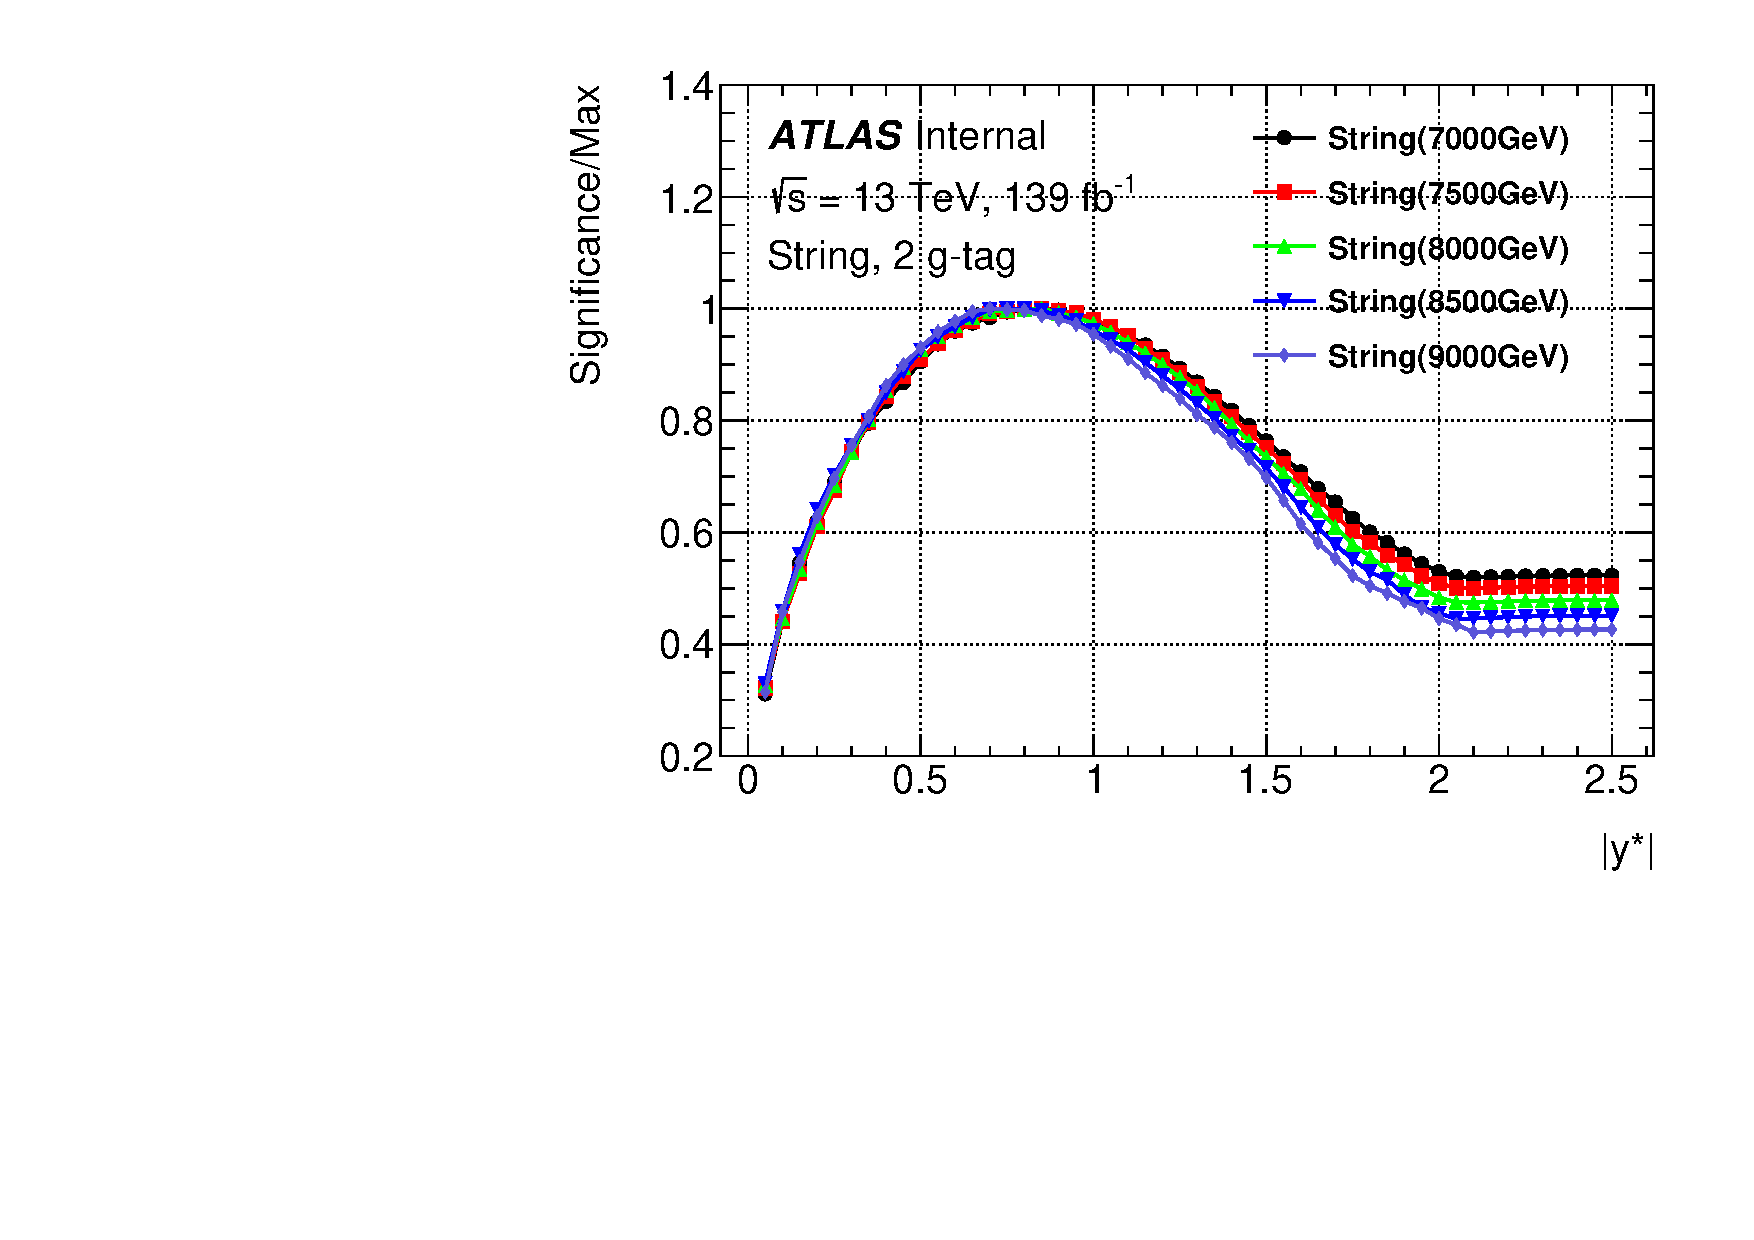
\includegraphics[width=0.48\columnwidth]{figures/yStarOptimization/Significance_String_gg.pdf}}
        \caption{String significance as a function \ystar\ cut in the case of (a) $\geq$1 g-tag, (b) 2 g-tag.}
        \label{fig: string significance as a function of y* cut}
\end{figure}

\subsection{dijet mass turn-on}
\label{section:dijetmassturn-on} % uncomment if label used.


The \mjj\ turn-on is measured using data by comparing events collected with the highest \pT\ 
trigger with one with a lower \pt\ threshold.  The efficiency for the HLT\_j420 trigger is calculated by comparing to the 
following triggers in each data taking period: 2015 HLT\_j360, 2016 HLT\_j380, 2017 and 2018 HLT\_mu50. We use a muon trigger 
2017 and 2018 as HLT\_j420 is the only unprescaled jet trigger available. Since the HLT\_mu50 is available for all running periods 
a comparison is made for the complete Run~2 data set. 
A mass cut will be applied to remove events where 
the trigger efficiency is less than 99.5\%.

Figure \ref{fig: mass turn-on yStar 0.6} shows the efficiencies as a function of \mjj\ for $|\ystar|<0.6$ in 
two g-tag regions for both triggers.  The results 
are summarised for data taking periods in Table~\ref{table:massTurnOns} and shown for the full Run~2 data 
taking period in Figures \ref{fig: mass turn-on yStar 0.6} and \ref{fig: mass turn-on yStar 0.8}. The detailed results for
each year are added to the Appendix~\ref{section:triggerturnon}.


The \mjj\ mass has been chosend to be slightly above th e value of the plateau ($\geq$99.5\%) and is 1100\,\GeV.
for $|\ystar|<0.6$ and 1200\,\GeV for $|\ystar|<0.6$ for samples with either one or two gluon tags.

\begin{table}[h]
	\centering 
		\caption{ The \mjj\ value of the plateau ($\geq$99.5\%) for each period of data taking. 
		\label{table:massTurnOns}
		}
	\begin{tabular}{SSSSS}
	\toprule
\multicolumn{1}{c}{Data Taking Period}  &  \multicolumn{2}{c}{Mass turn on $|\ystar|<0.6$ } &  \multicolumn{2}{c}{Mass turn on $|\ystar|<0.8$ } \\
 & \multicolumn{1}{c}{$\geq$1 g-tag (\GeV )} &  \multicolumn{1}{c}{2 g-tag (\GeV )} 
 & \multicolumn{1}{c}{$\geq$1 g-tag (\GeV )} &  \multicolumn{1}{c}{2 g-tag (\GeV )}  \\
\midrule 
2015  & 1040 & 1030 & 1160 & 1160 \\
2016  & 1030 & 1030 & 1160 & 1170 \\
2017  & 990 & 1000  & 1110 & 1120 \\
2018  & 1000 & 1010  & 1110 & 1120 \\
\multicolumn{1}{c}{Run~2} & 1020 & 1030 & 1120 & 1120 \\
\bottomrule
\end{tabular}
\end{table}


\begin{figure}[htbp]
        \centering
        \subfigure[$\geq$1 g-tag]{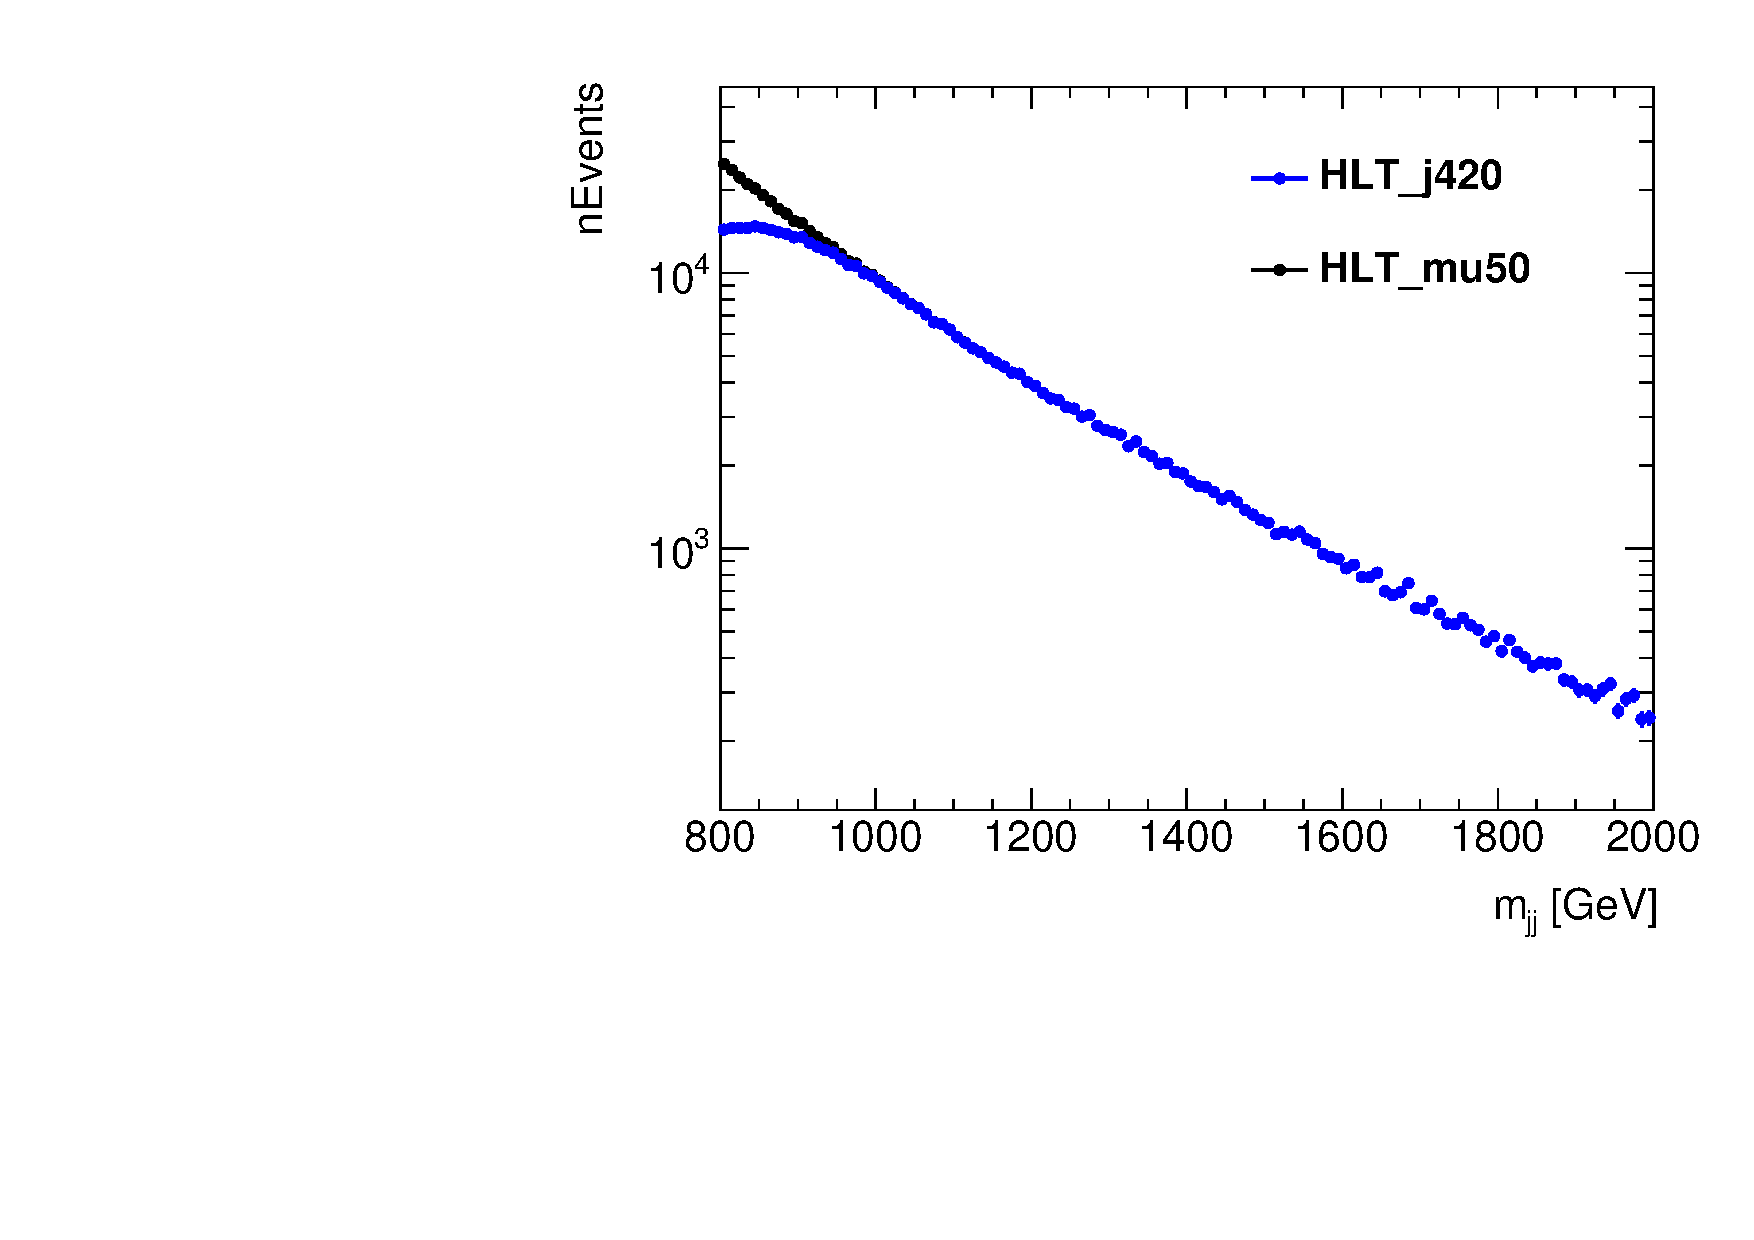
\includegraphics[width=0.48\columnwidth]{figures/massturnon/yStar0p6/mjj_turnon_1gluonTag_yStar0p6}}
        \subfigure[2 g-tag]{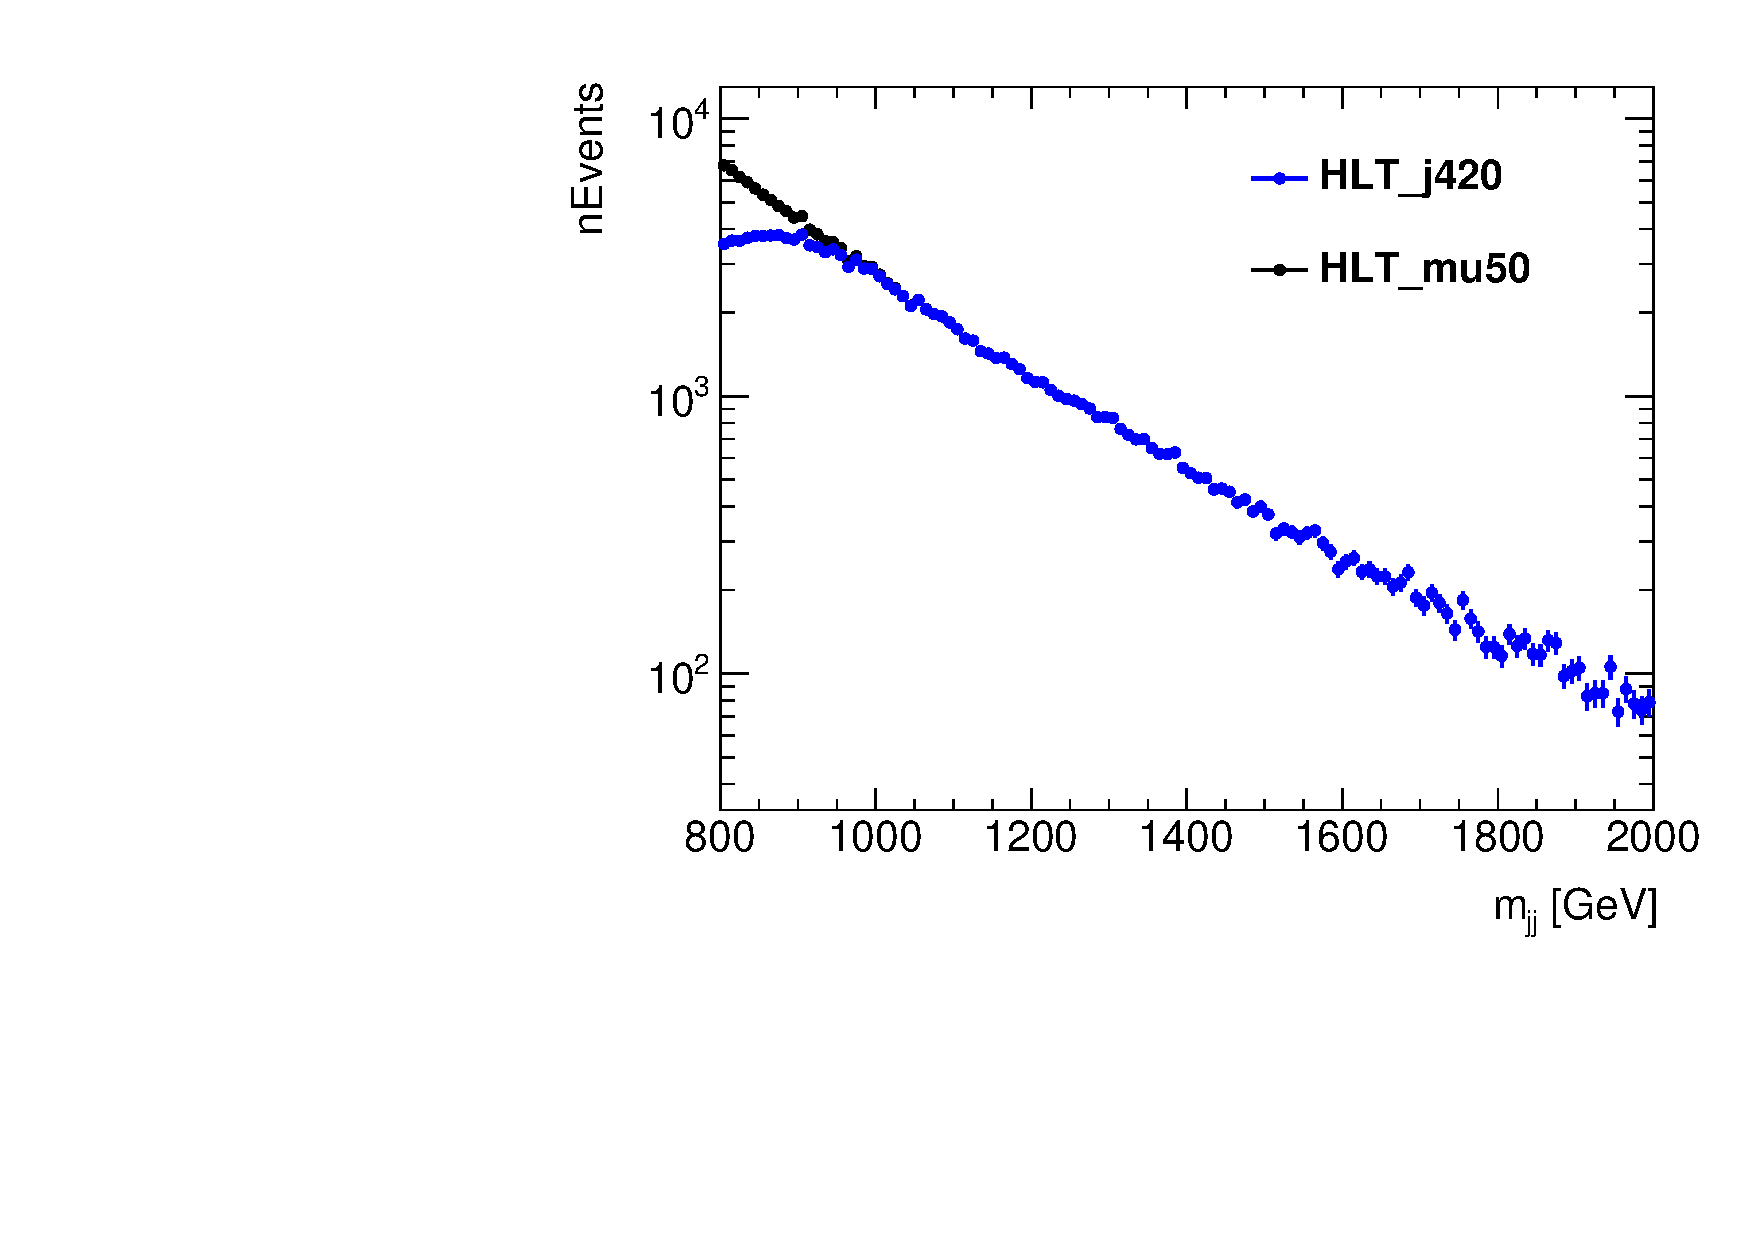
\includegraphics[width=0.48\columnwidth]{figures/massturnon/yStar0p6/mjj_turnon_2gluonTag_yStar0p6}}
        \\
        \subfigure[$\geq$1 g-tag]{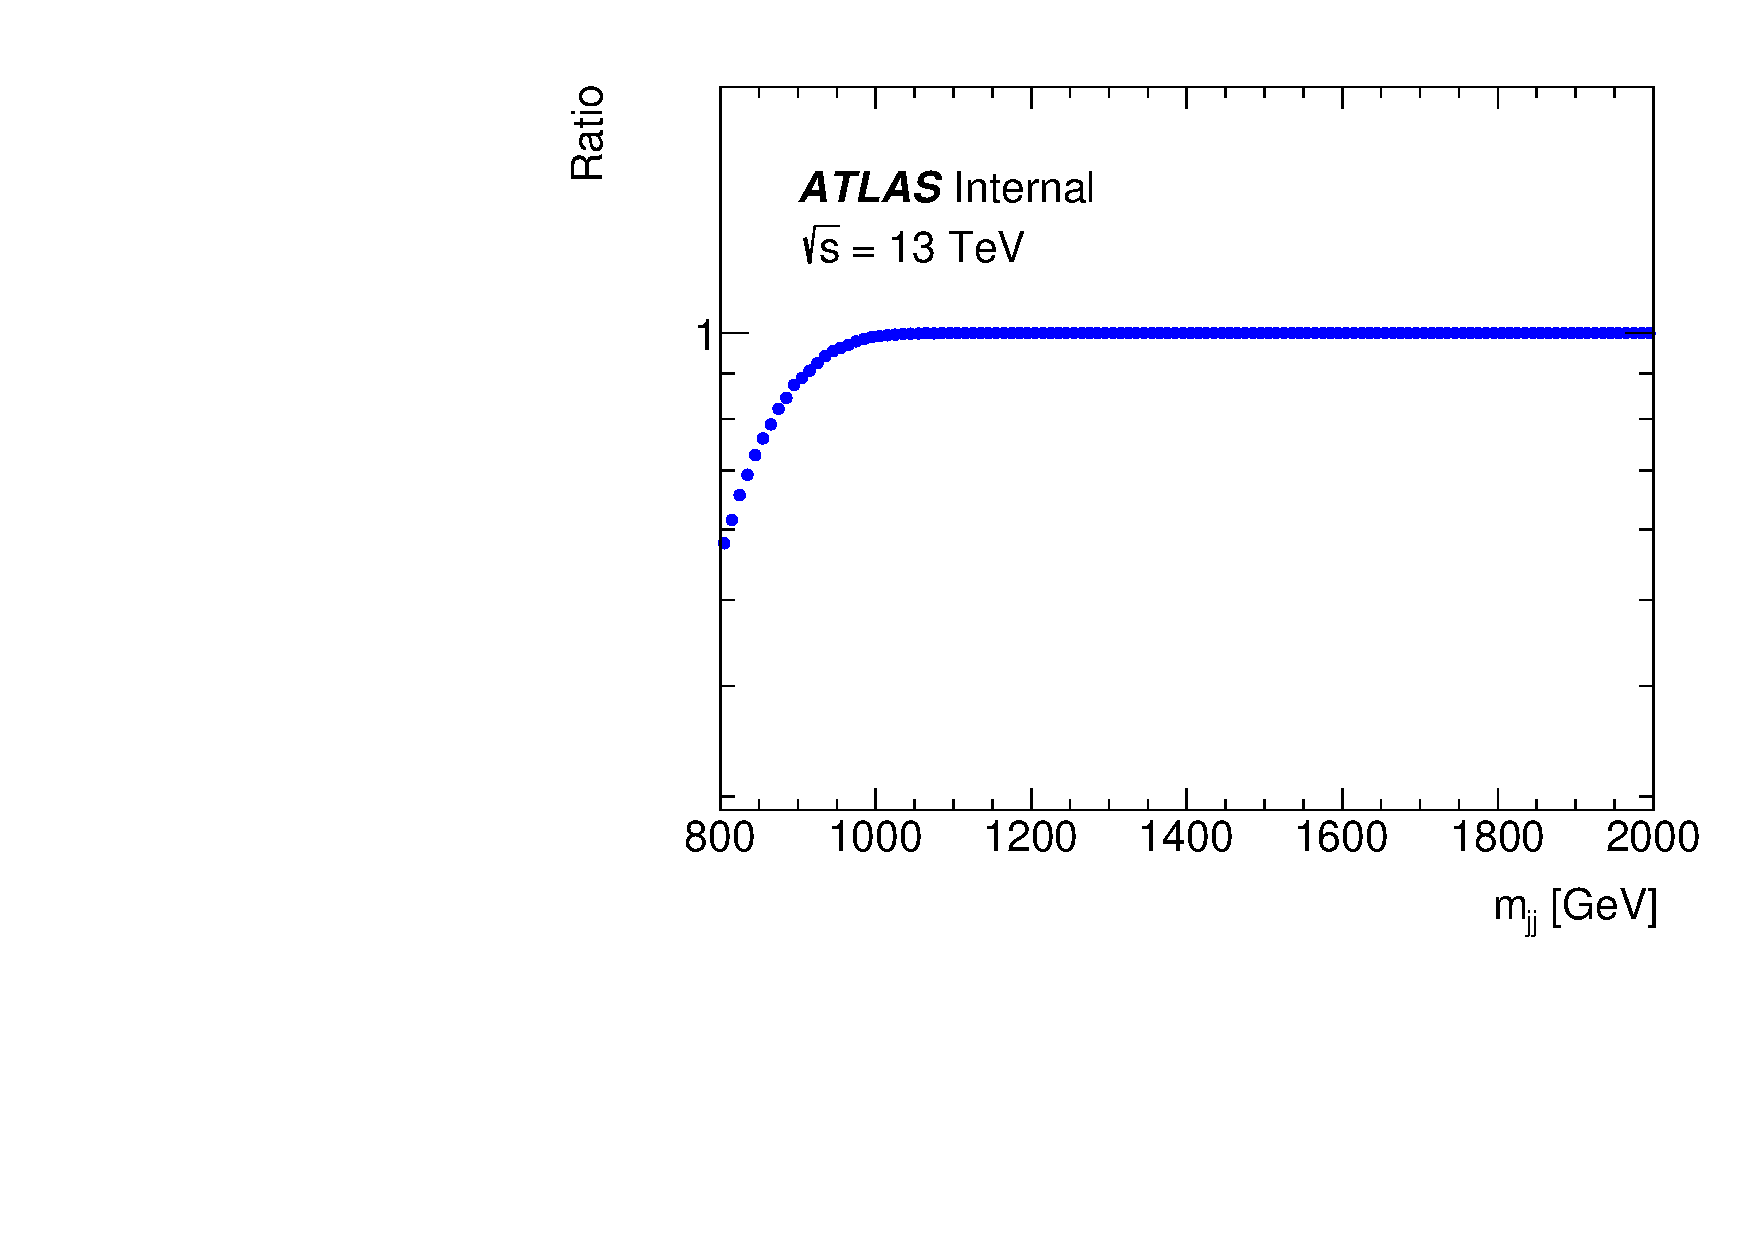
\includegraphics[width=0.48\columnwidth]{figures/massturnon/yStar0p6/Ratio_mjj_turnon_1gluonTag_yStar0p6}}
        \subfigure[2 g-tag]{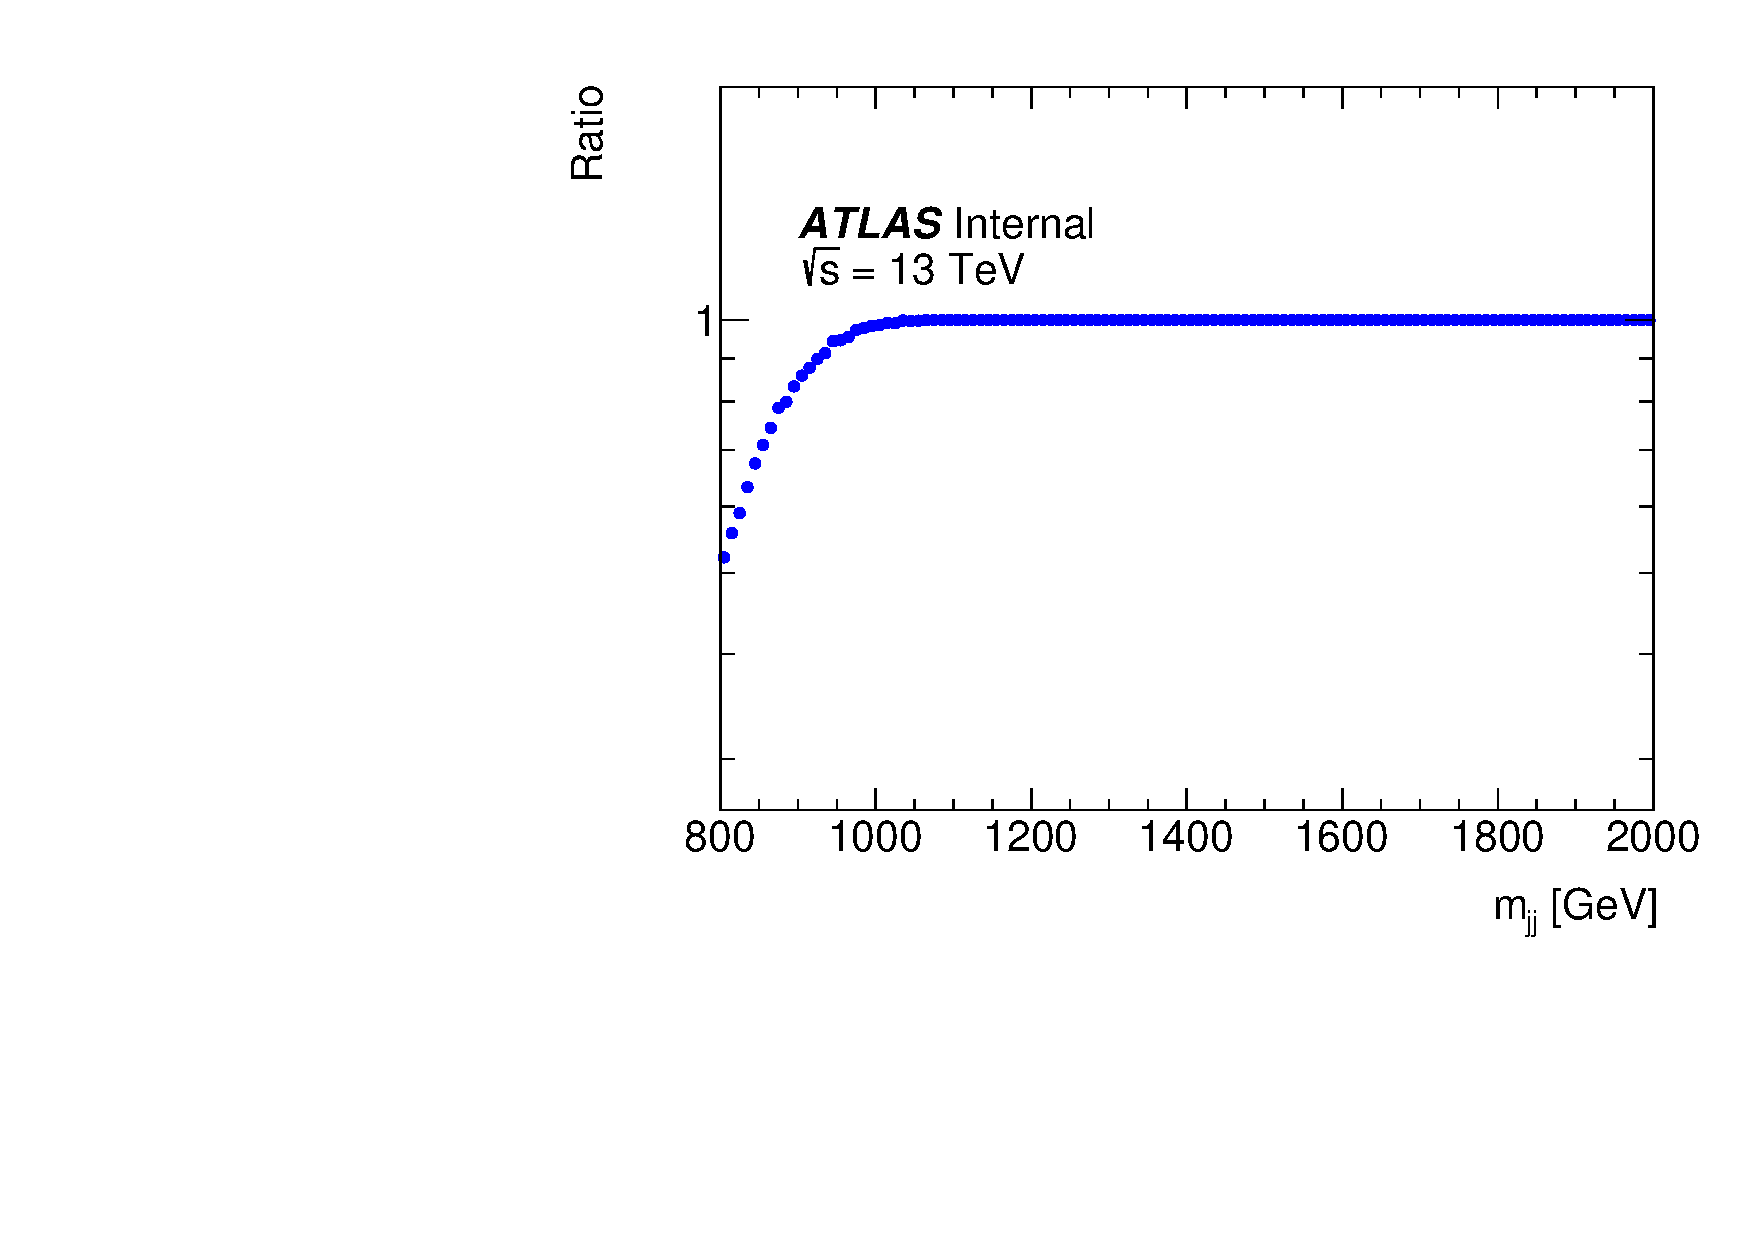
\includegraphics[width=0.48\columnwidth]{figures/massturnon/yStar0p6/Ratio_mjj_turnon_2gluonTag_yStar0p6}}
        
        \caption{Efficiencies as a function of \mjj\ for $|\ystar|<0.6$ using HLT\_j420 compared with HLT\_mu50 in the case of comparison of mass spectra with 
        (a) $\geq$1 g-tag, (b) 2 g-tag and the ratio between the two (c) $\geq$1 g-tag and (d) 2 g-tag.}
        \label{fig: mass turn-on yStar 0.6}
\end{figure}

\begin{figure}[htbp]
        \centering
        \subfigure[$\geq$1 g-tag]{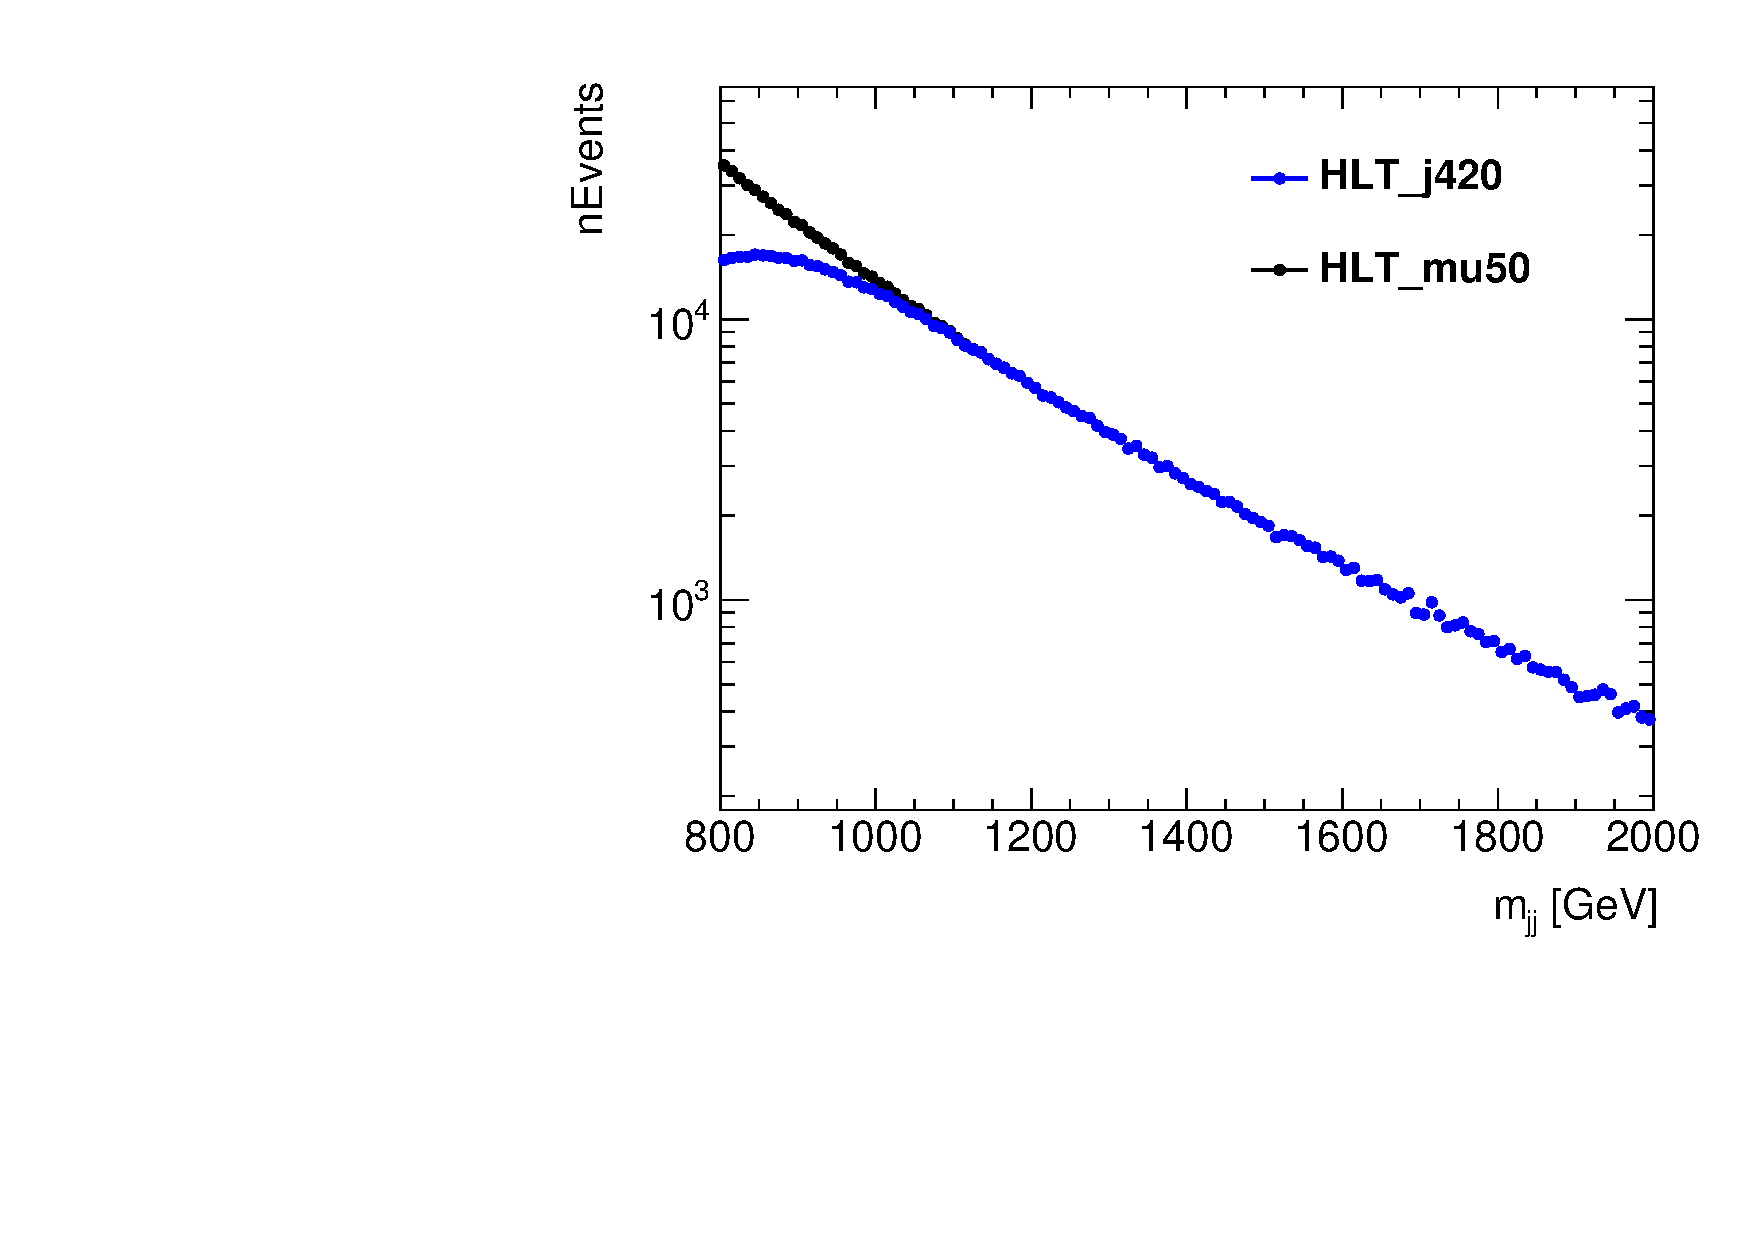
\includegraphics[width=0.48\columnwidth]{figures/massturnon/yStar0p8/mjj_turnon_1gluonTag_yStar0p8}}
        \subfigure[2 g-tag]{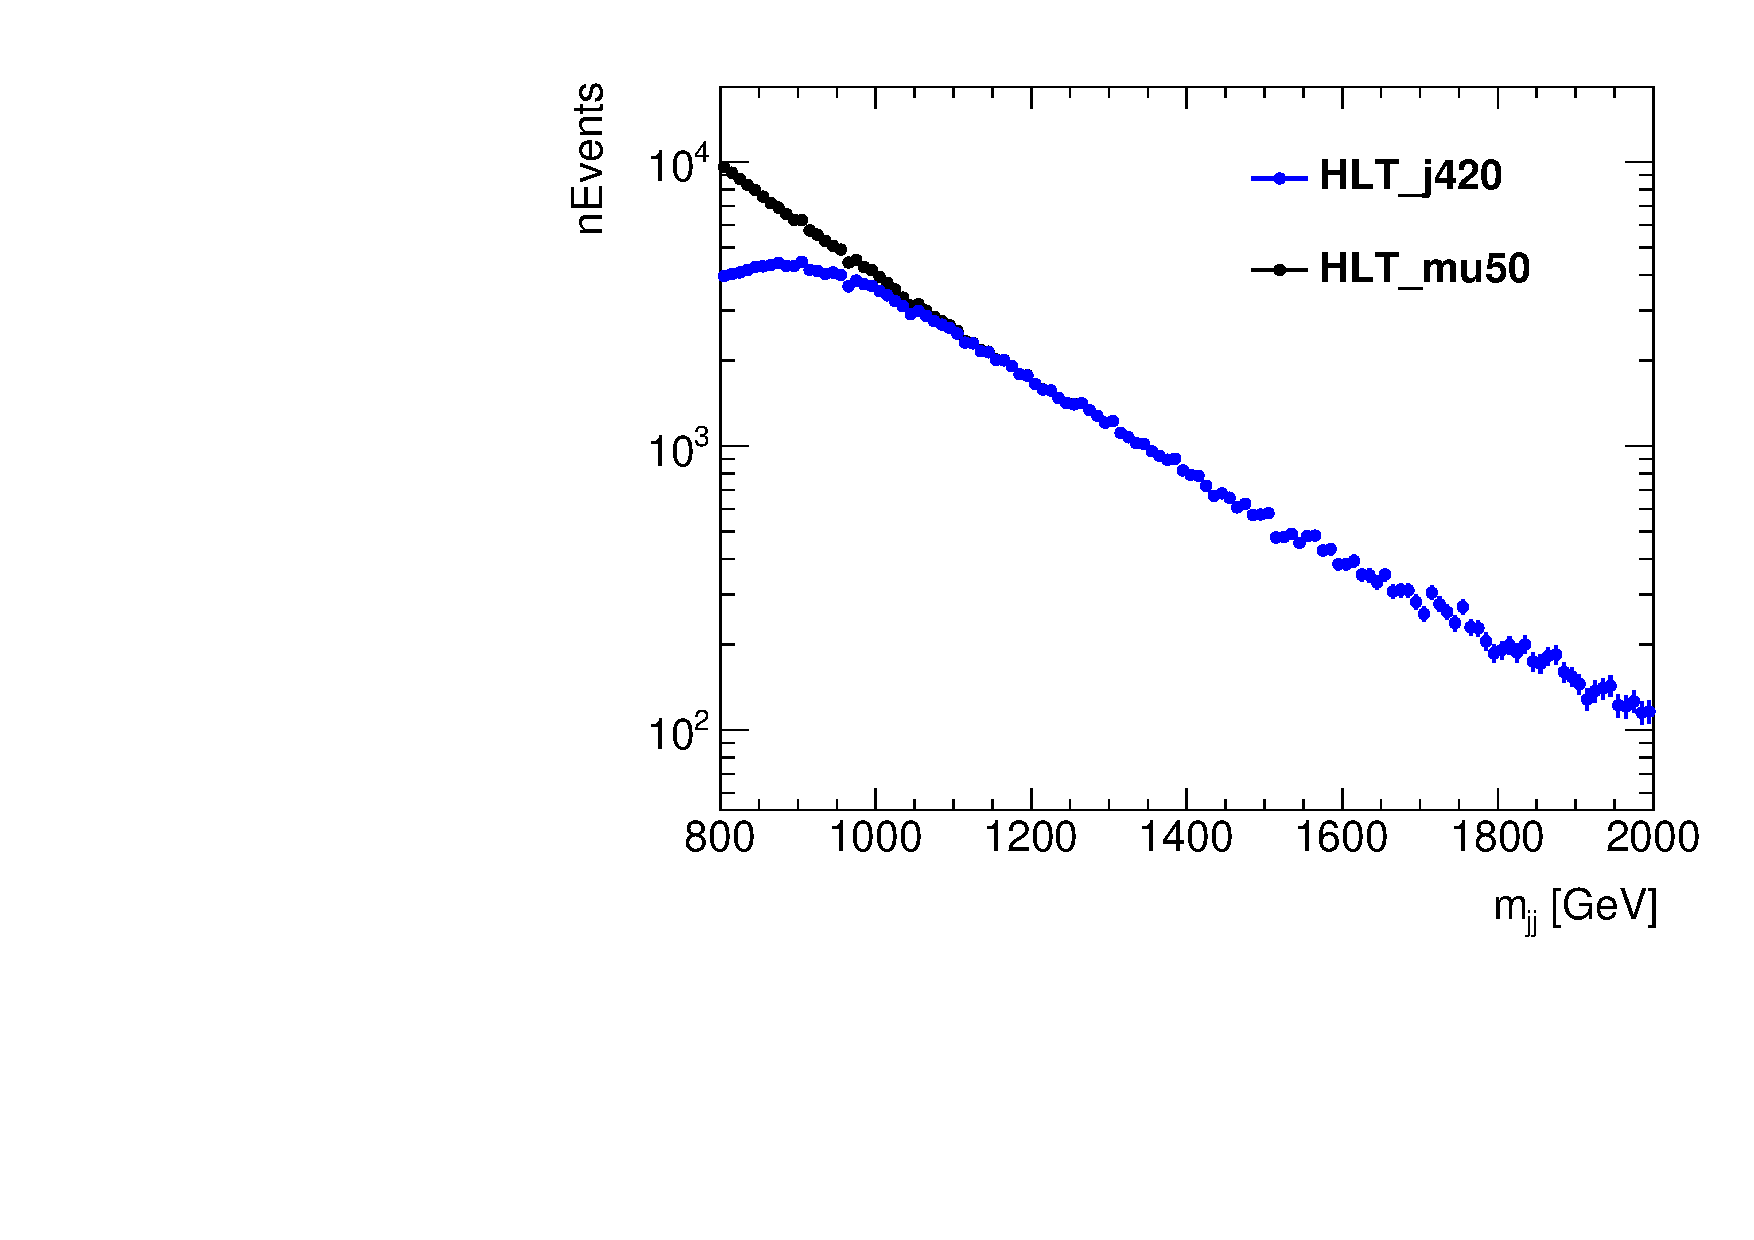
\includegraphics[width=0.48\columnwidth]{figures/massturnon/yStar0p8/mjj_turnon_2gluonTag_yStar0p8}}
        \\
        \subfigure[$\geq$1 g-tag]{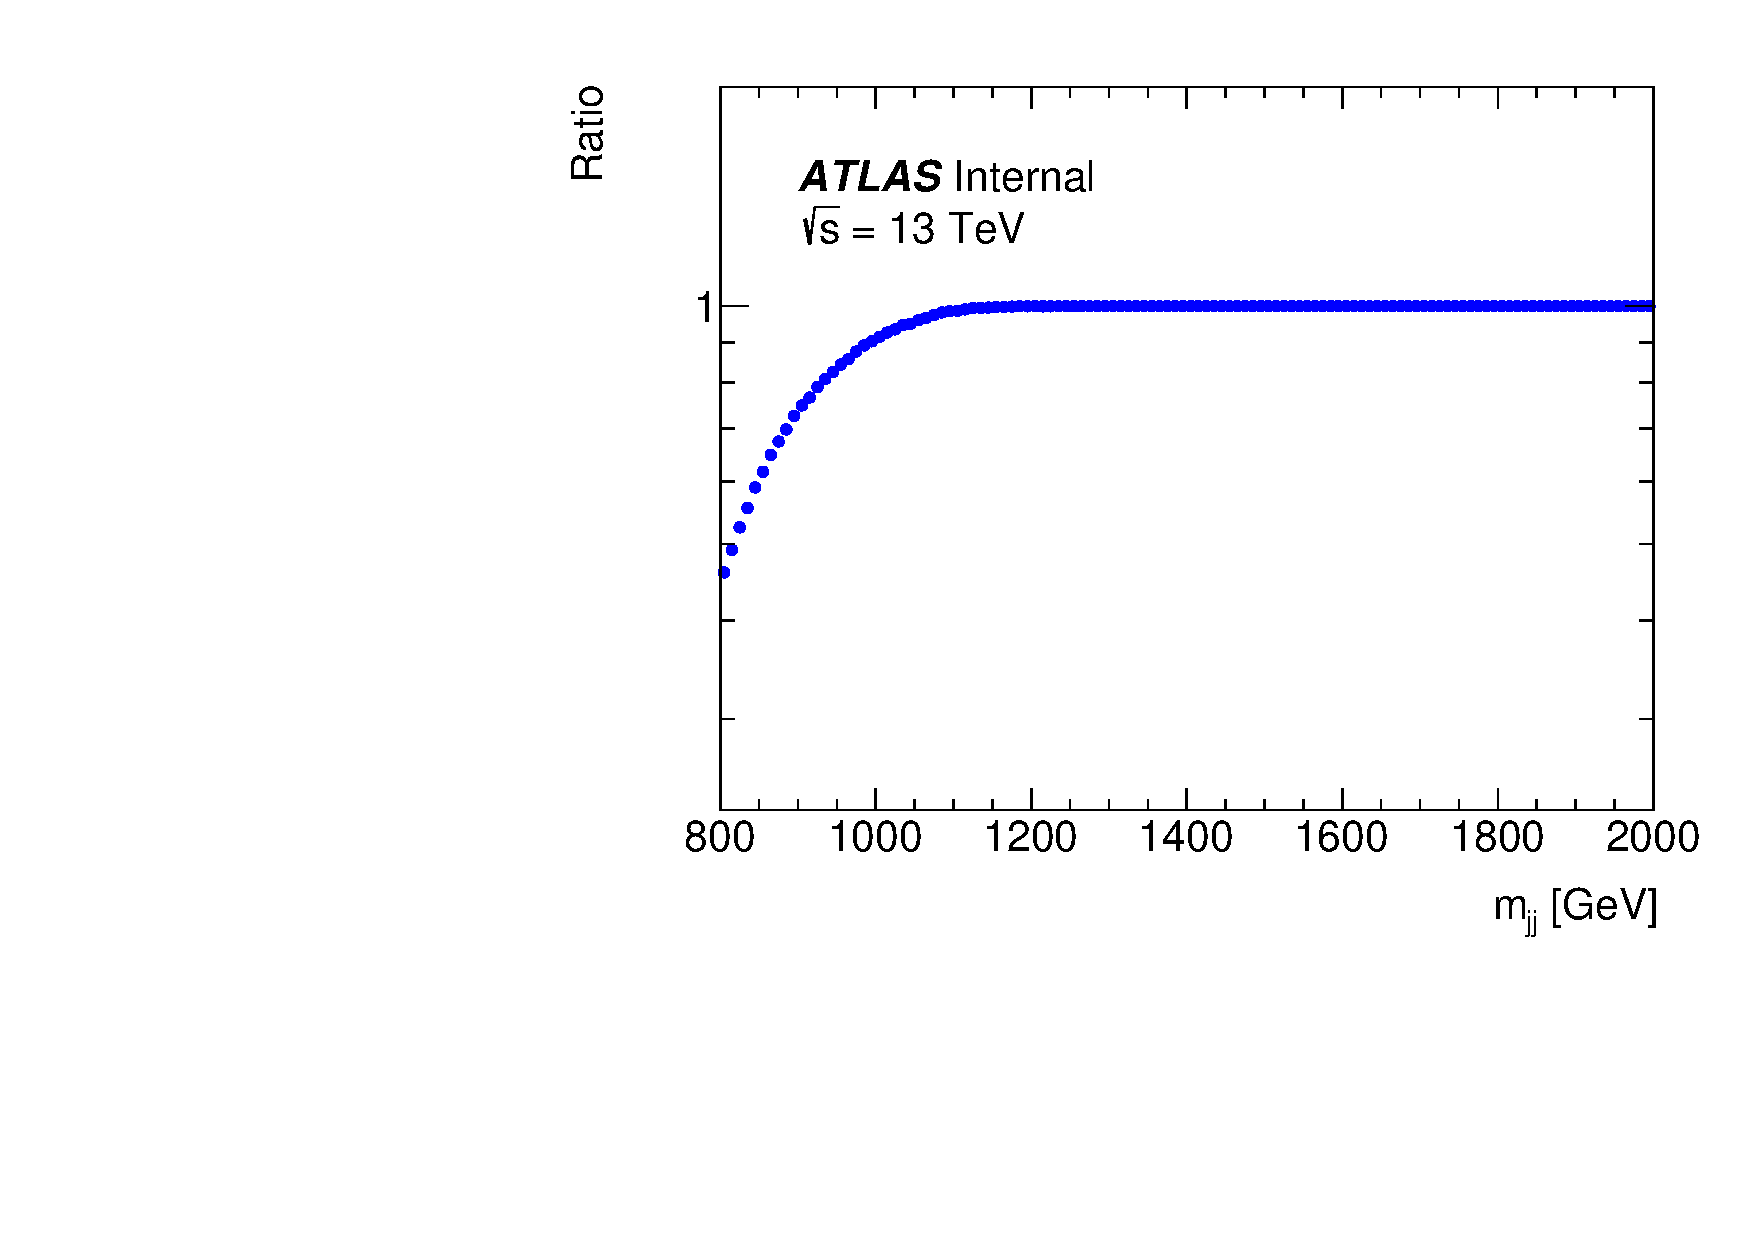
\includegraphics[width=0.48\columnwidth]{figures/massturnon/yStar0p8/Ratio_mjj_turnon_1gluonTag_yStar0p8}}
        \subfigure[2 g-tag]{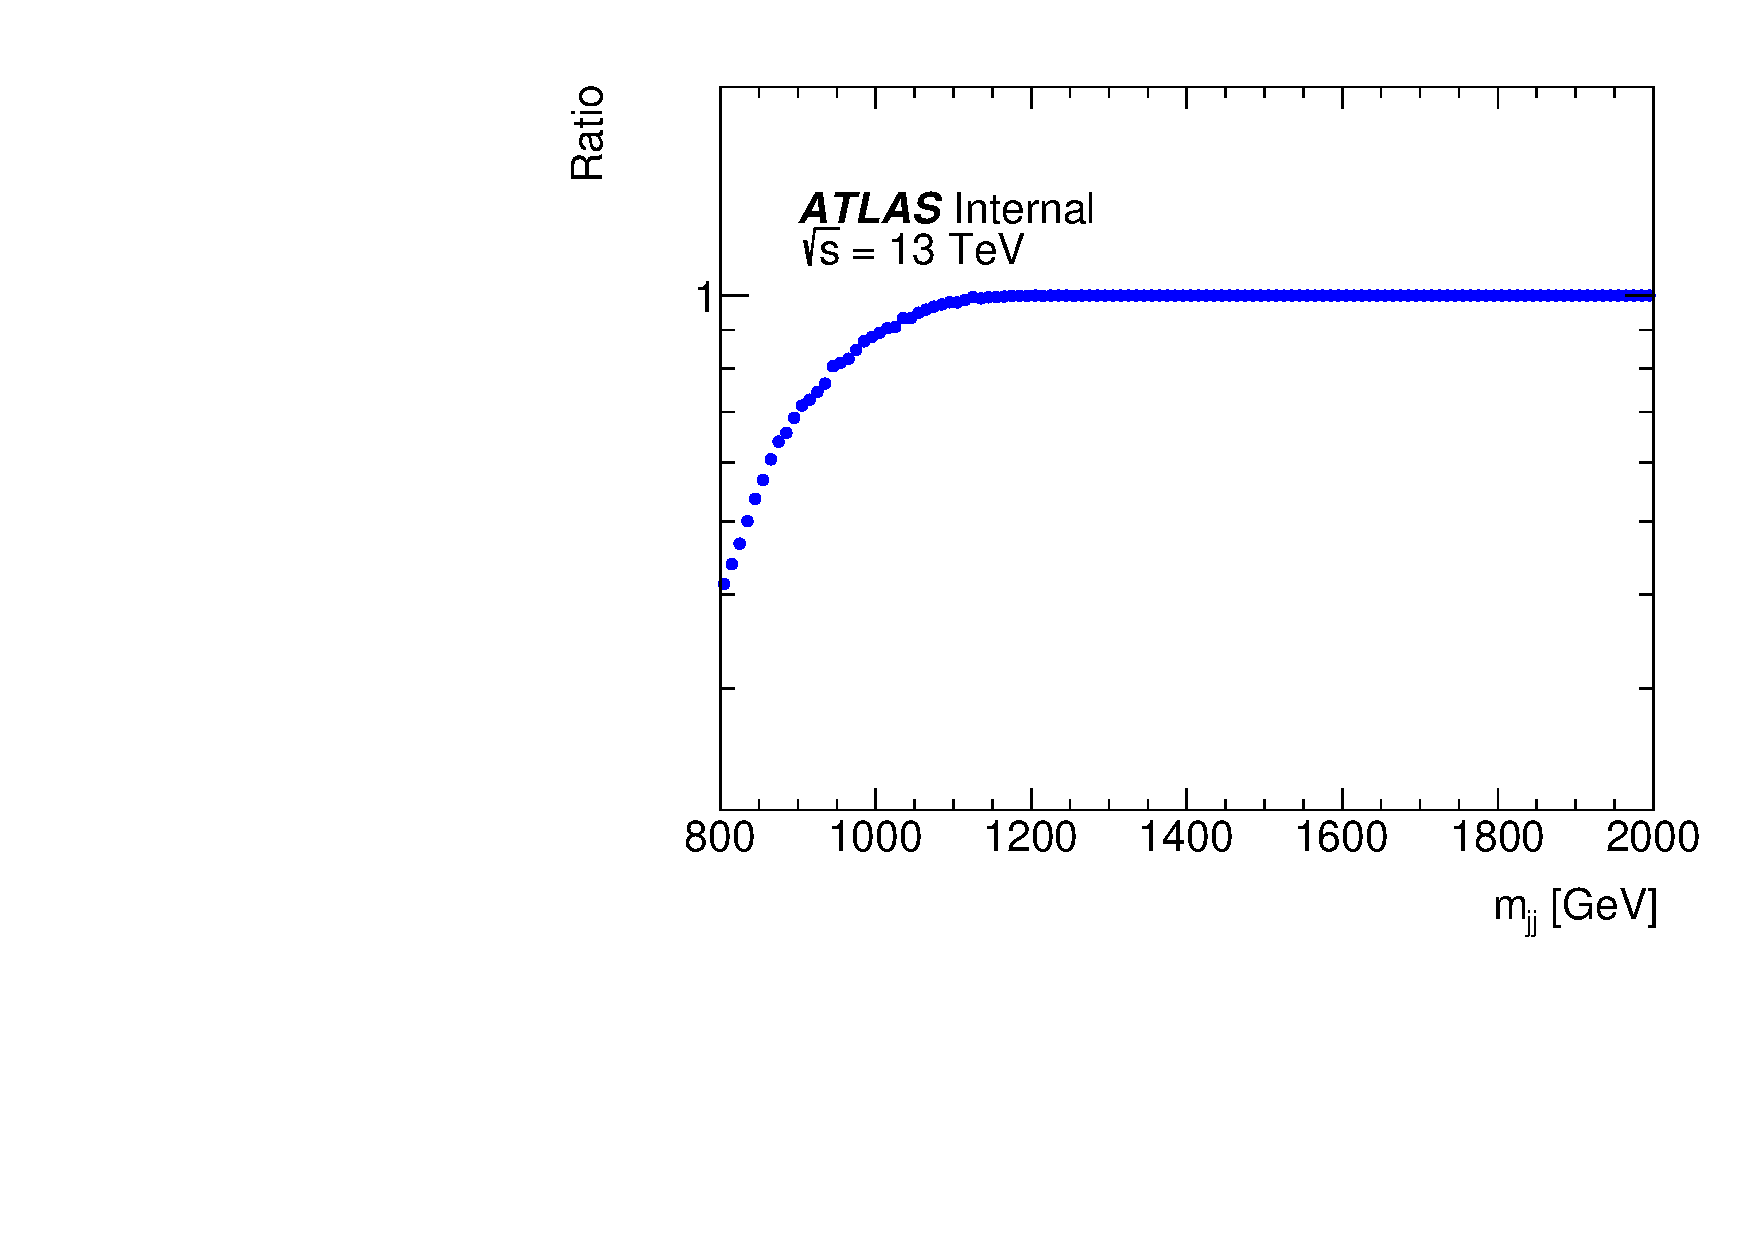
\includegraphics[width=0.48\columnwidth]{figures/massturnon/yStar0p8/Ratio_mjj_turnon_2gluonTag_yStar0p8}}
        \caption{Efficiencies as a function of \mjj\ for $|\ystar|<0.8$ using HLT\_j420 compared with HLT\_mu50 in the case of comparison of mass spectra with 
        (a) $\geq$1 g-tag, (b) 2 g-tag and the ratio between the two (c) $\geq$1 g-tag and (d) 2 g-tag.}
        \label{fig: mass turn-on yStar 0.8}
\end{figure}




\subsection{Optimised selection}

In addition to the baseline selection cuts described in Section~\ref{sec:base_selection}, 
the following cuts are applied to different regions to optimize the
search potential and to ensure good tracking efficiency. 

The following additional cuts are applied to the H$^\prime$ search.
\begin{itemize}
\item $|\ystar| < 0.6$
\item $\mjj > 1100\,\GeV$
\end{itemize}

The following additional cuts are applied to the string resonance search.
\begin{itemize}
\item $|\ystar| < 0.8$
\item $\mjj > 1200\,\GeV$
\end{itemize}

The above cuts define the inclusive samples.
The following additional cuts are for quark-gluon tagging.
\begin{itemize}
\item $|\eta| < 2.1$ (both jets)
\item $\ge 1$ gluon tagged (75\% working point)
\item 2 gluons tagged (75\% working point)
\end{itemize}

\noindent
where the 75\% gluon selection criteria is $n_\mathrm{track} > -7.3 + 4.2\ln(\pt)$.

The cutflow tables obtained on full
Run-2 data are presented in Table~\ref{tab:data1518totalcutflow} in Appendix~\ref{section:cutflow}, where as Tables~\ref{tab:data2015cutflow}-~\ref{tab:data2018cutflow} presents the cutflow separately for each year between 2015-2018. 
The tables ~\ref{tab:bckgdcutflowMC16aWeighted} - ~\ref{tab:bckgdcutflowMC16eWeighted} in Appendix~\ref{section:cutflow} shows the cutflows 
obtained on Pythia QCD MC separated into campaigns MC16a, MC16d and MC16e. The numbers shown in these tables 
are weighted events normalised to the luminosity corresponding to each subcampaign.


\subsection{Basic kinematic plots}
%\label{sec:kinematic_distributions} % uncomment if label used.

\subsection{Gluon-Gluon Data Selection}

In this section a selection of kinematic and monitoring plots produced with the gluon-gluon sample selection on the full dataset is shown 
(Figures~\ref{fig:GGmonitoring1}, \ref{fig:GGmonitoring2}, \ref{fig:GGmonitoring3}. 


\begin{figure}[htb]
 \centering
 \subfigure[] {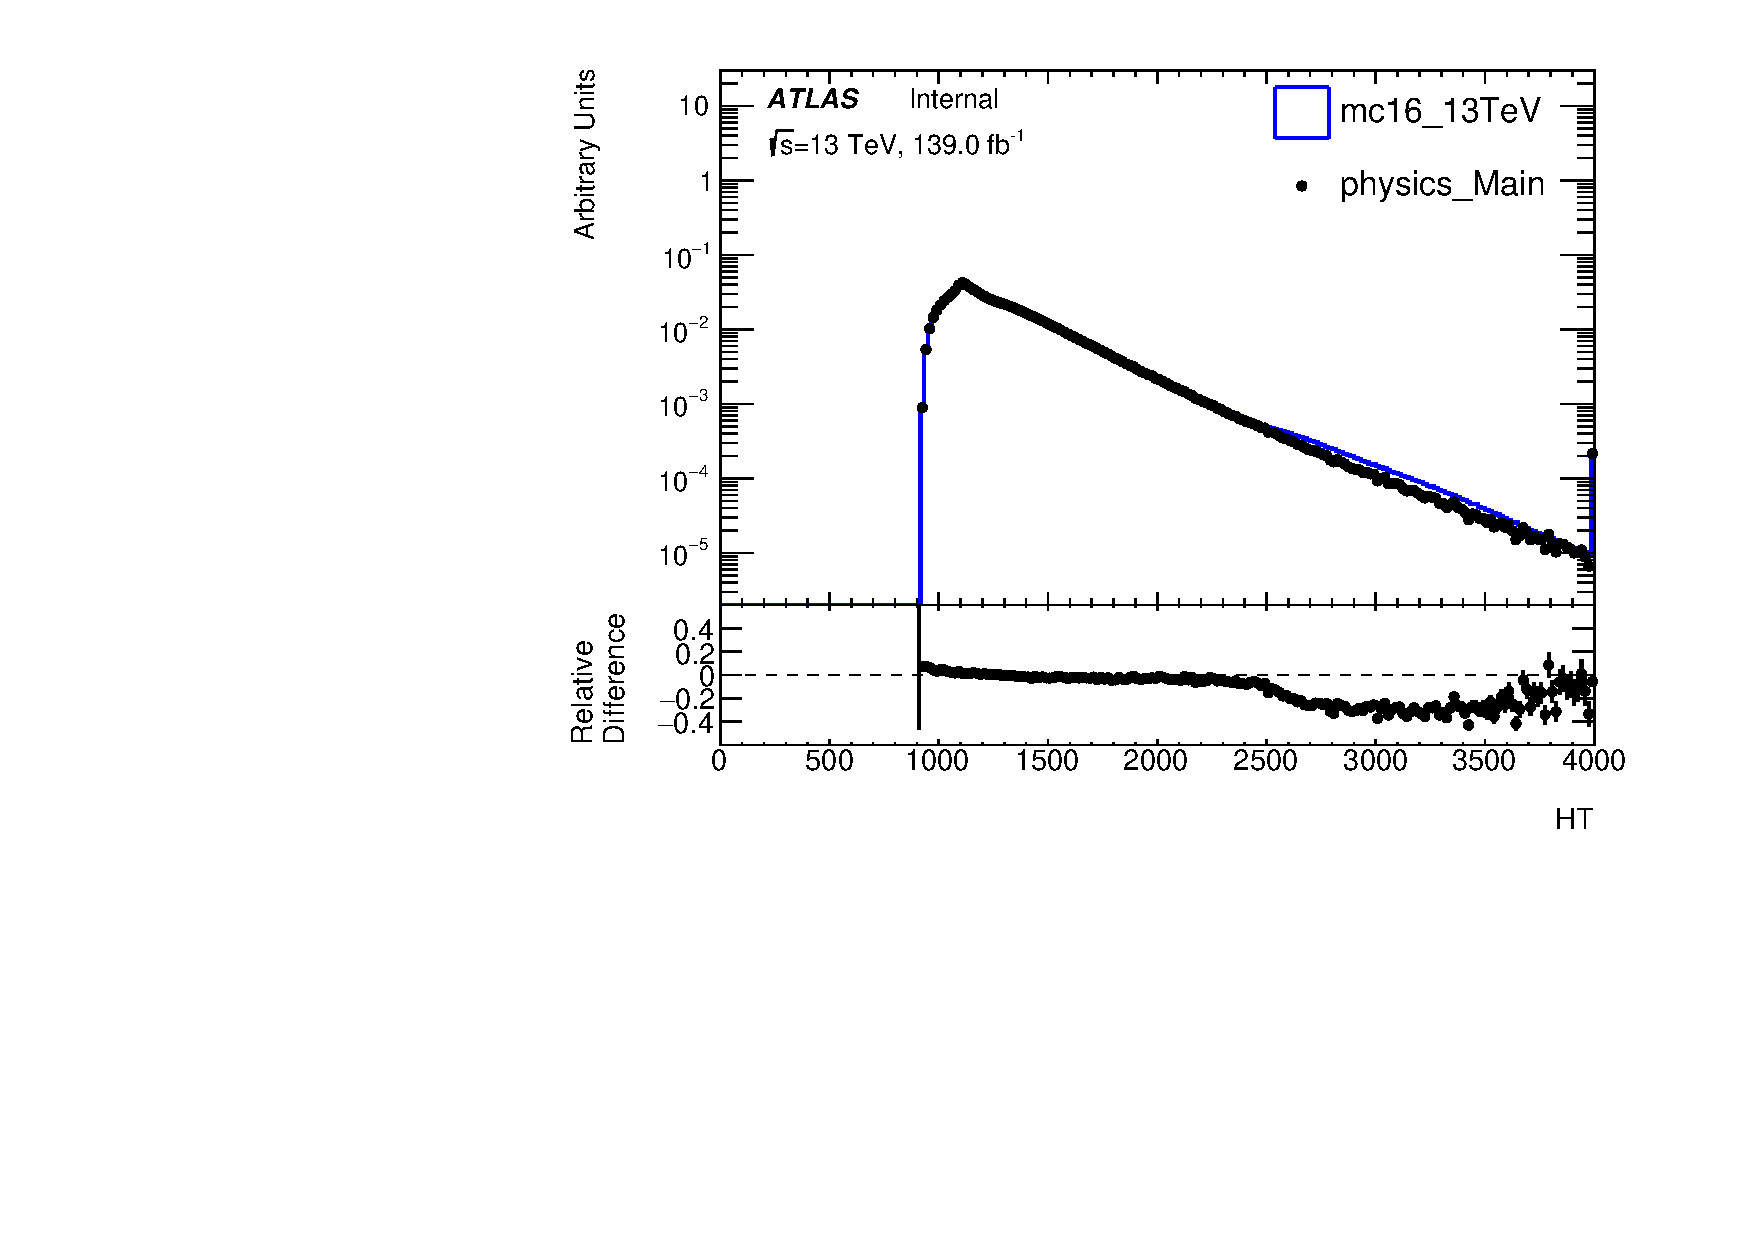
\includegraphics[width=0.45\textwidth]{figures/monitoring/GG/newStudy_HT_logY_v01.pdf}}
 \subfigure[] {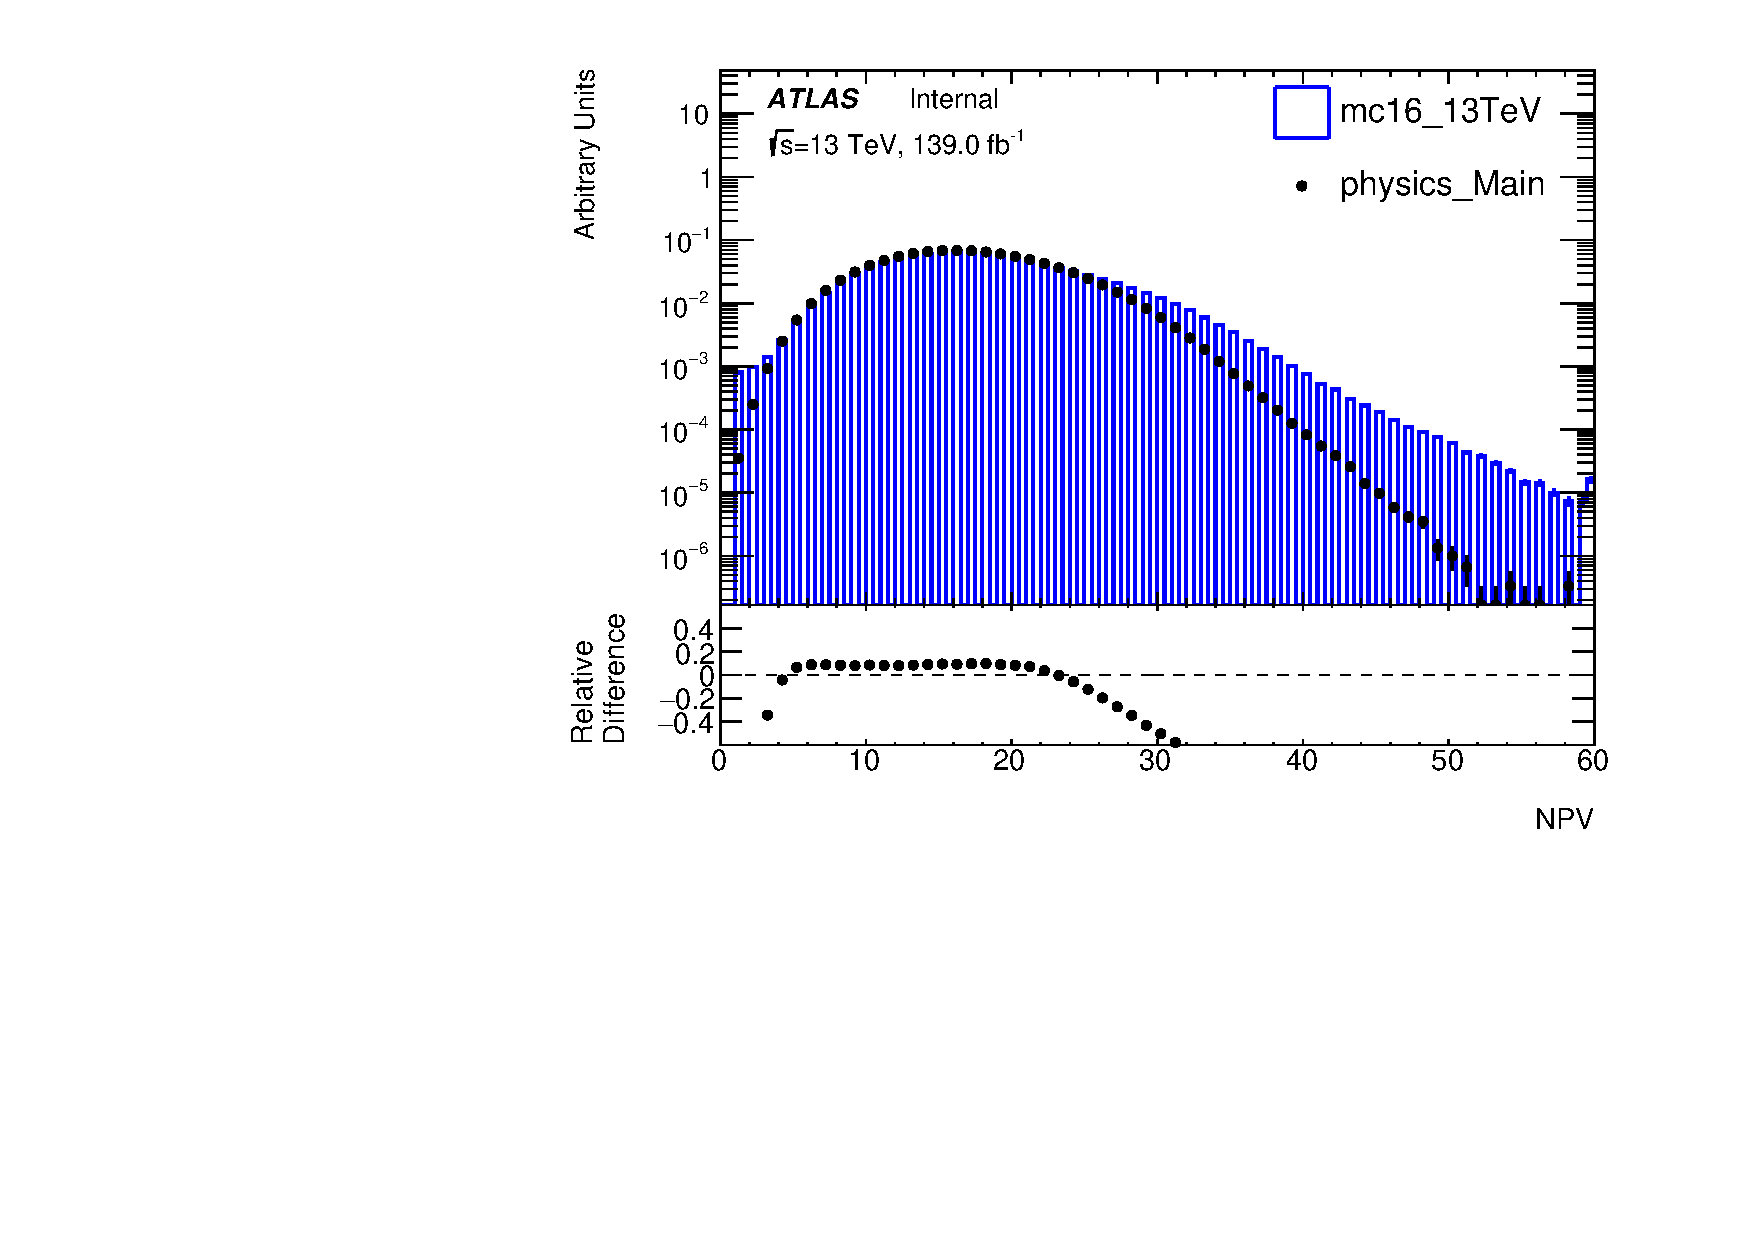
\includegraphics[width=0.45\textwidth]{figures/monitoring/GG/newStudy_NPV_logY_v01.pdf}}
 \subfigure[] {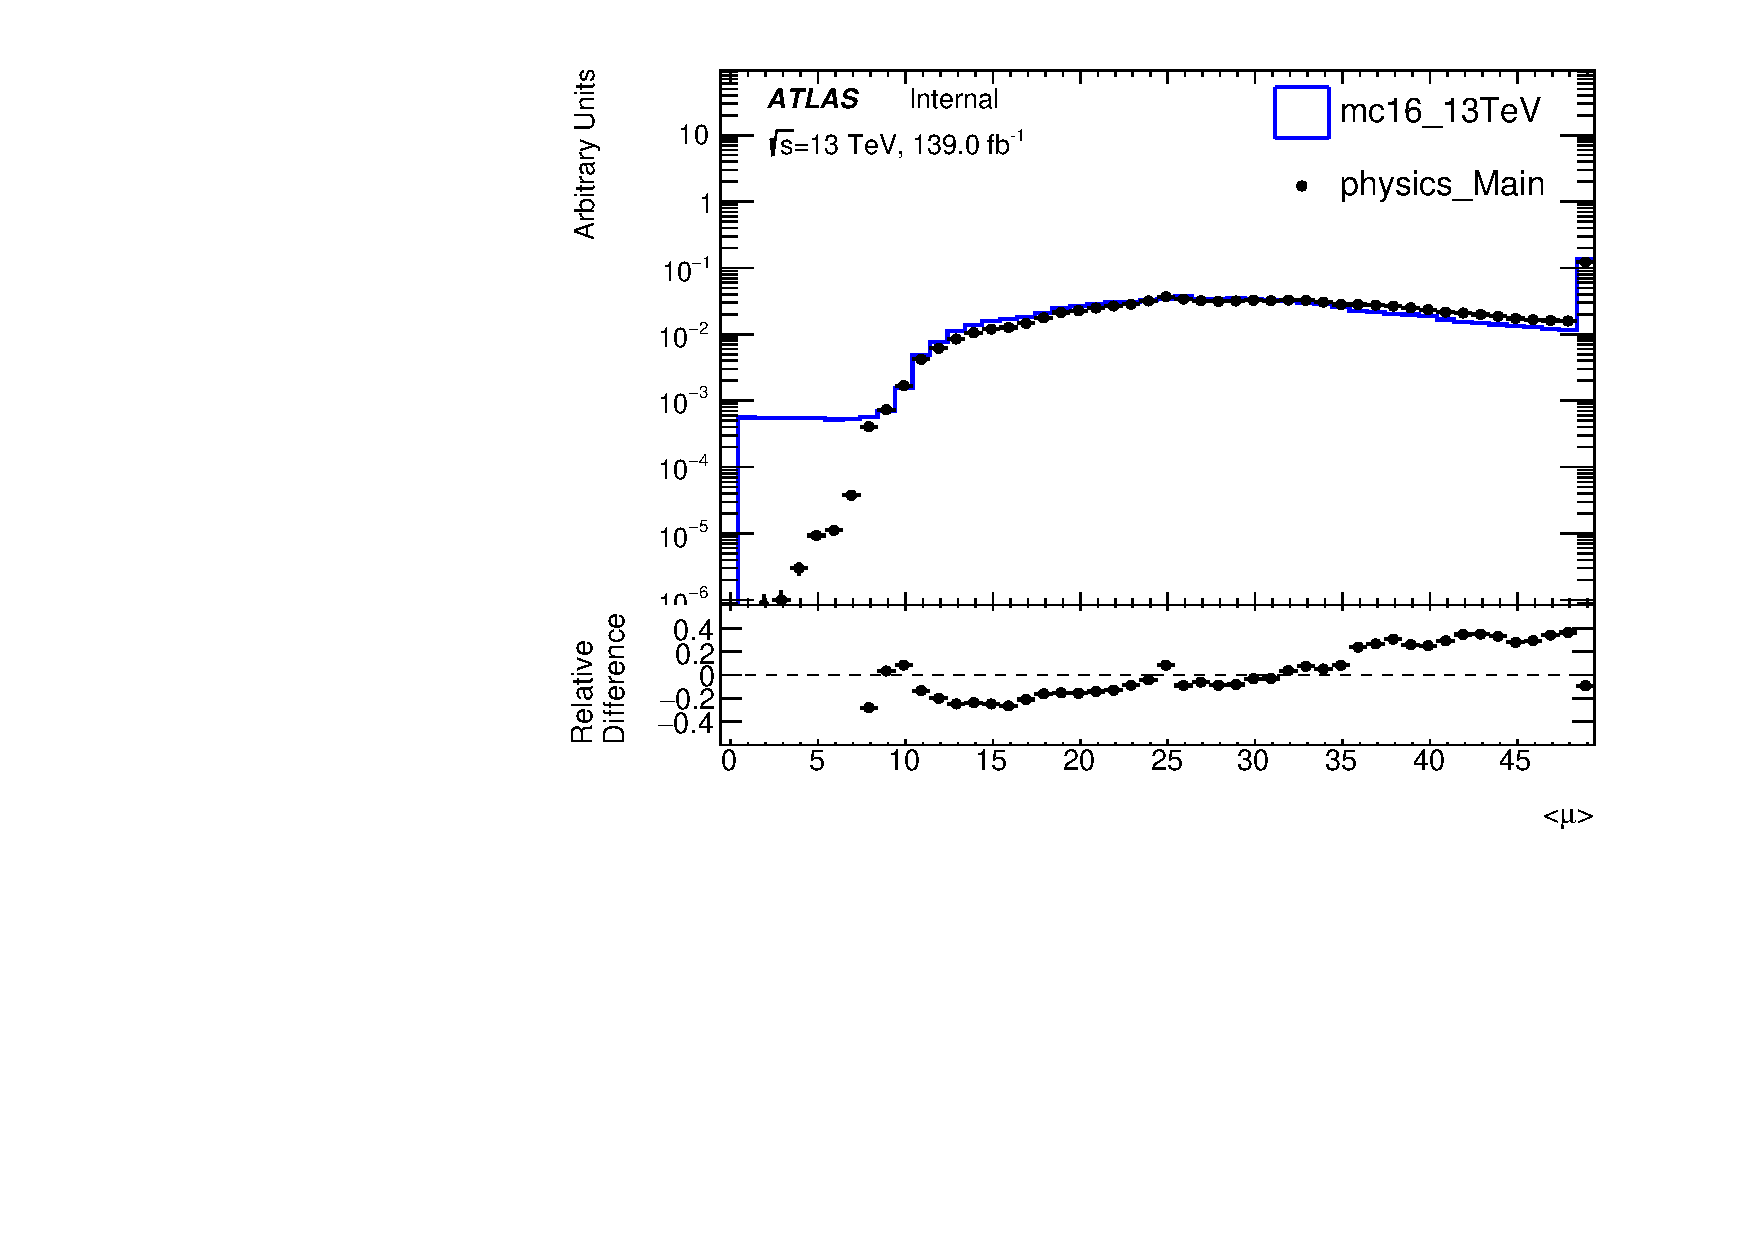
\includegraphics[width=0.45\textwidth]{figures/monitoring/GG/newStudy_averageInteractionsPerCrossing_logY_v01.pdf}}
  \subfigure[] {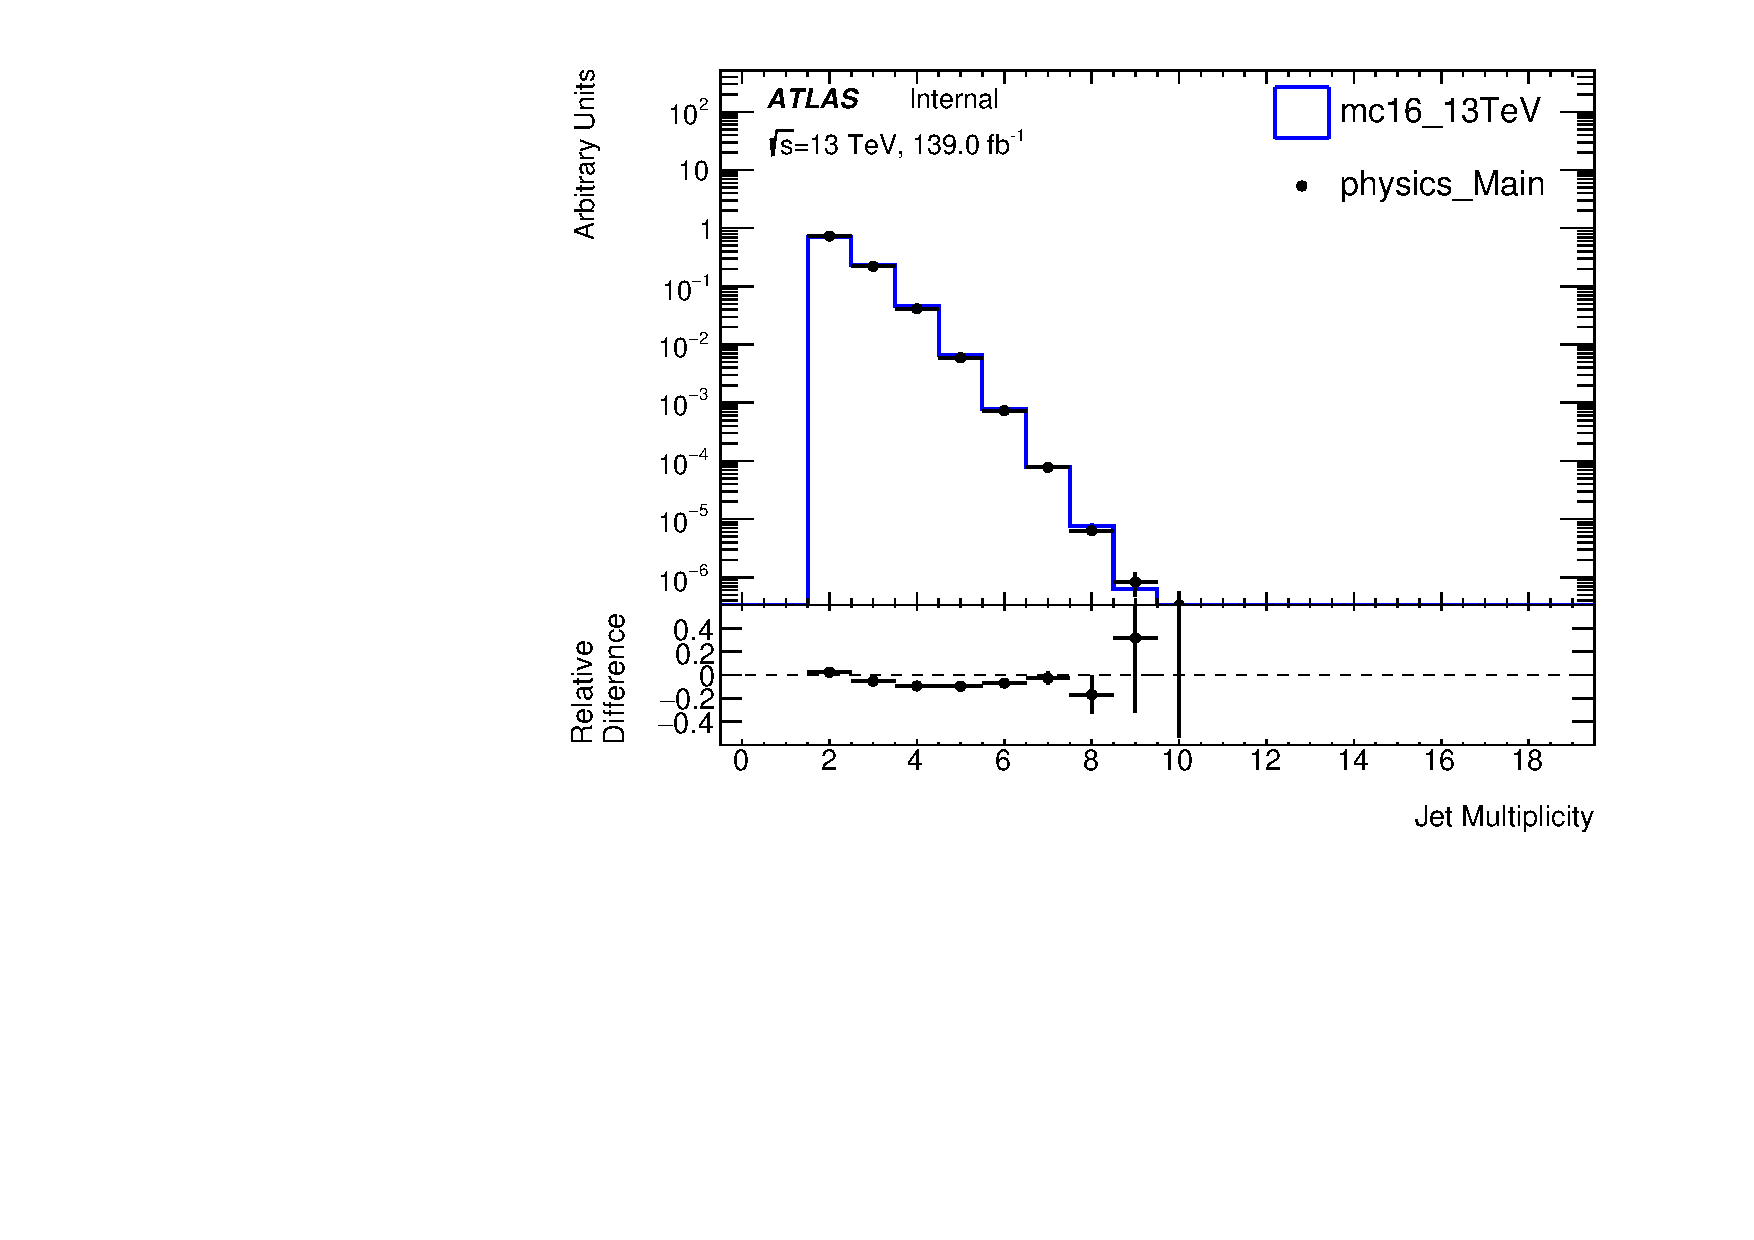
\includegraphics[width=0.45\textwidth]{figures/monitoring/GG/newStudy_njets_logY_v01.pdf}}
 \caption{Monitoring plots on %2016 data, 
 the gluon-gluon sample. (a) $H_T$, %(b) $MH_T$ (missing transverse momentum calculated only from the jets in the event), 
 (b) number of primary interaction vertices,
 (c) average interactions per bunch crossing, and 
 (d) number of jets.}
 \label{fig:GGmonitoring1}
\end{figure}

 \begin{figure}[htb]
 \centering
 \subfigure[] {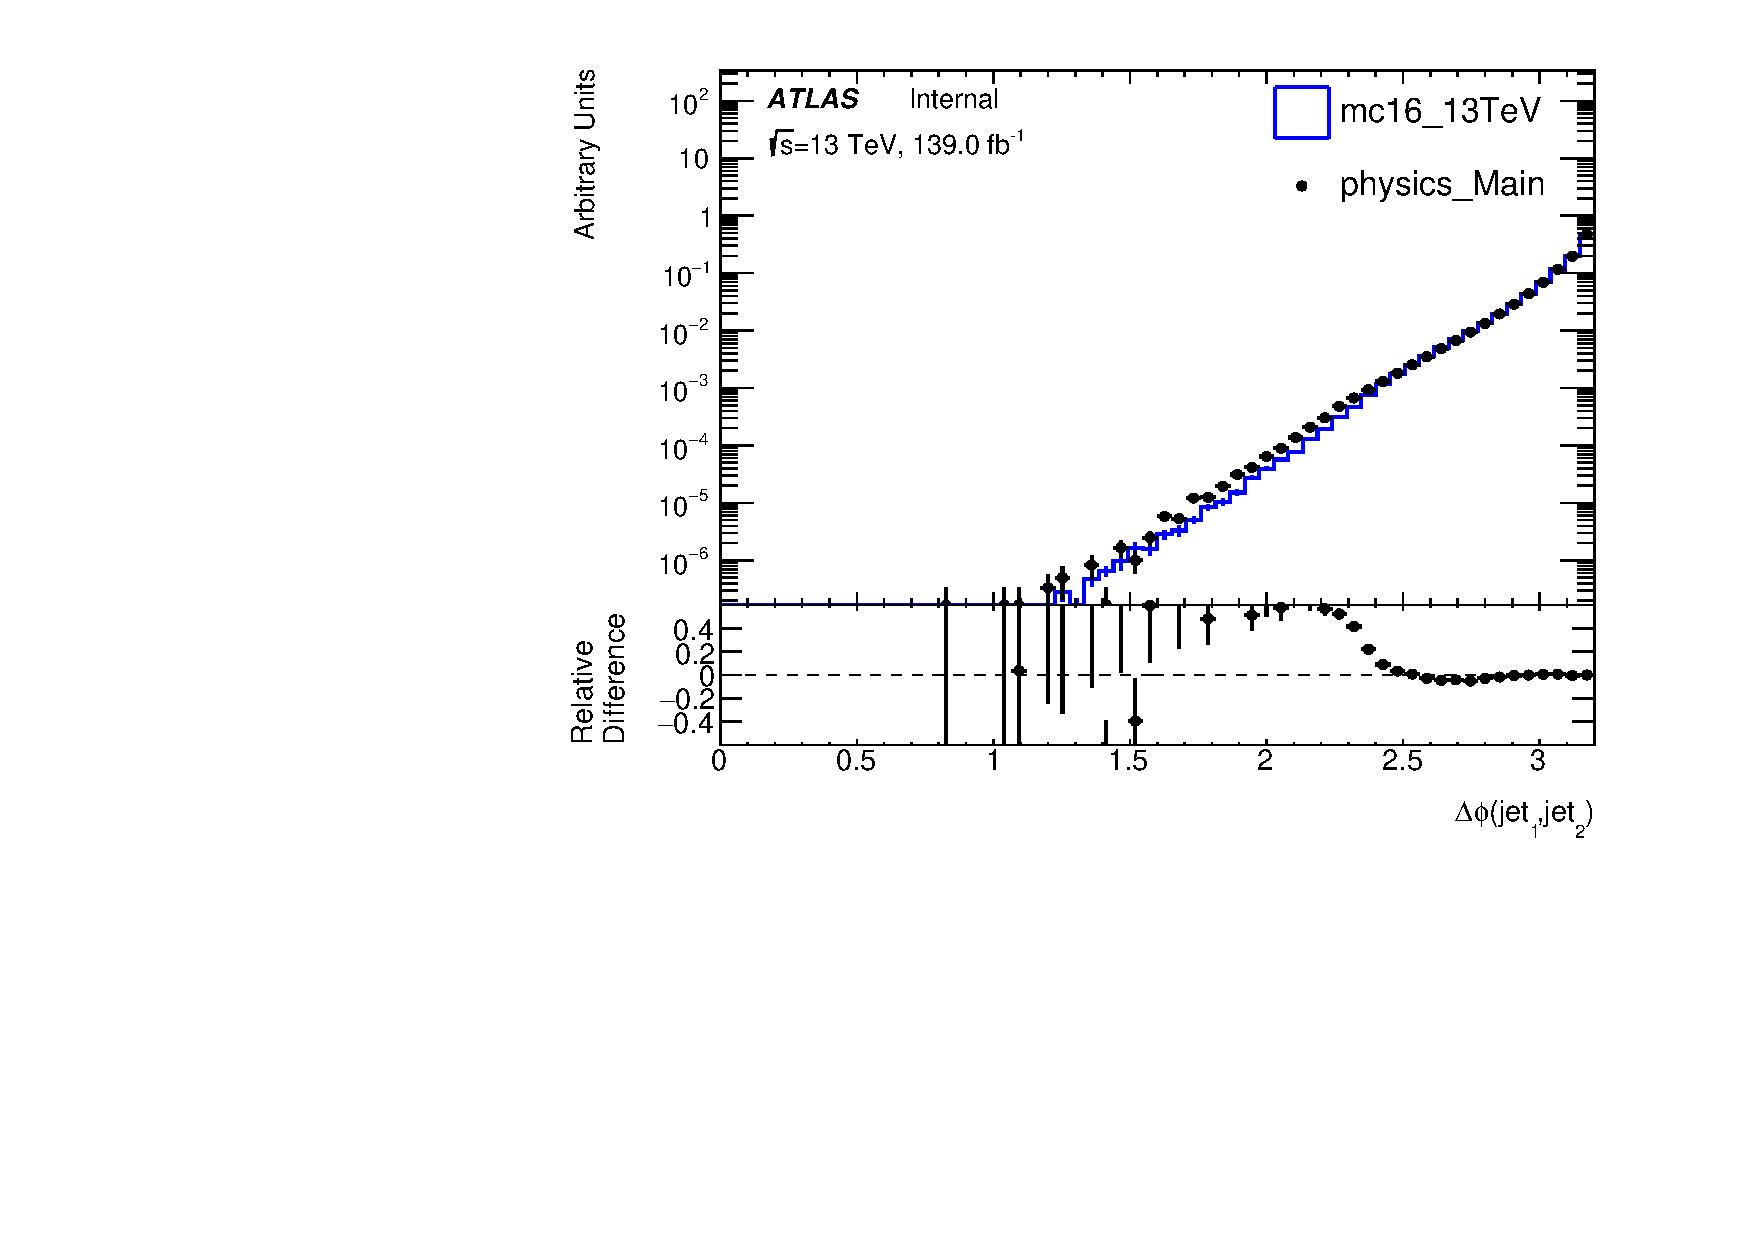
\includegraphics[width=0.45\textwidth]{figures/monitoring/GG/newStudy_deltaPhi_logY_v01.pdf}}
 \subfigure[] {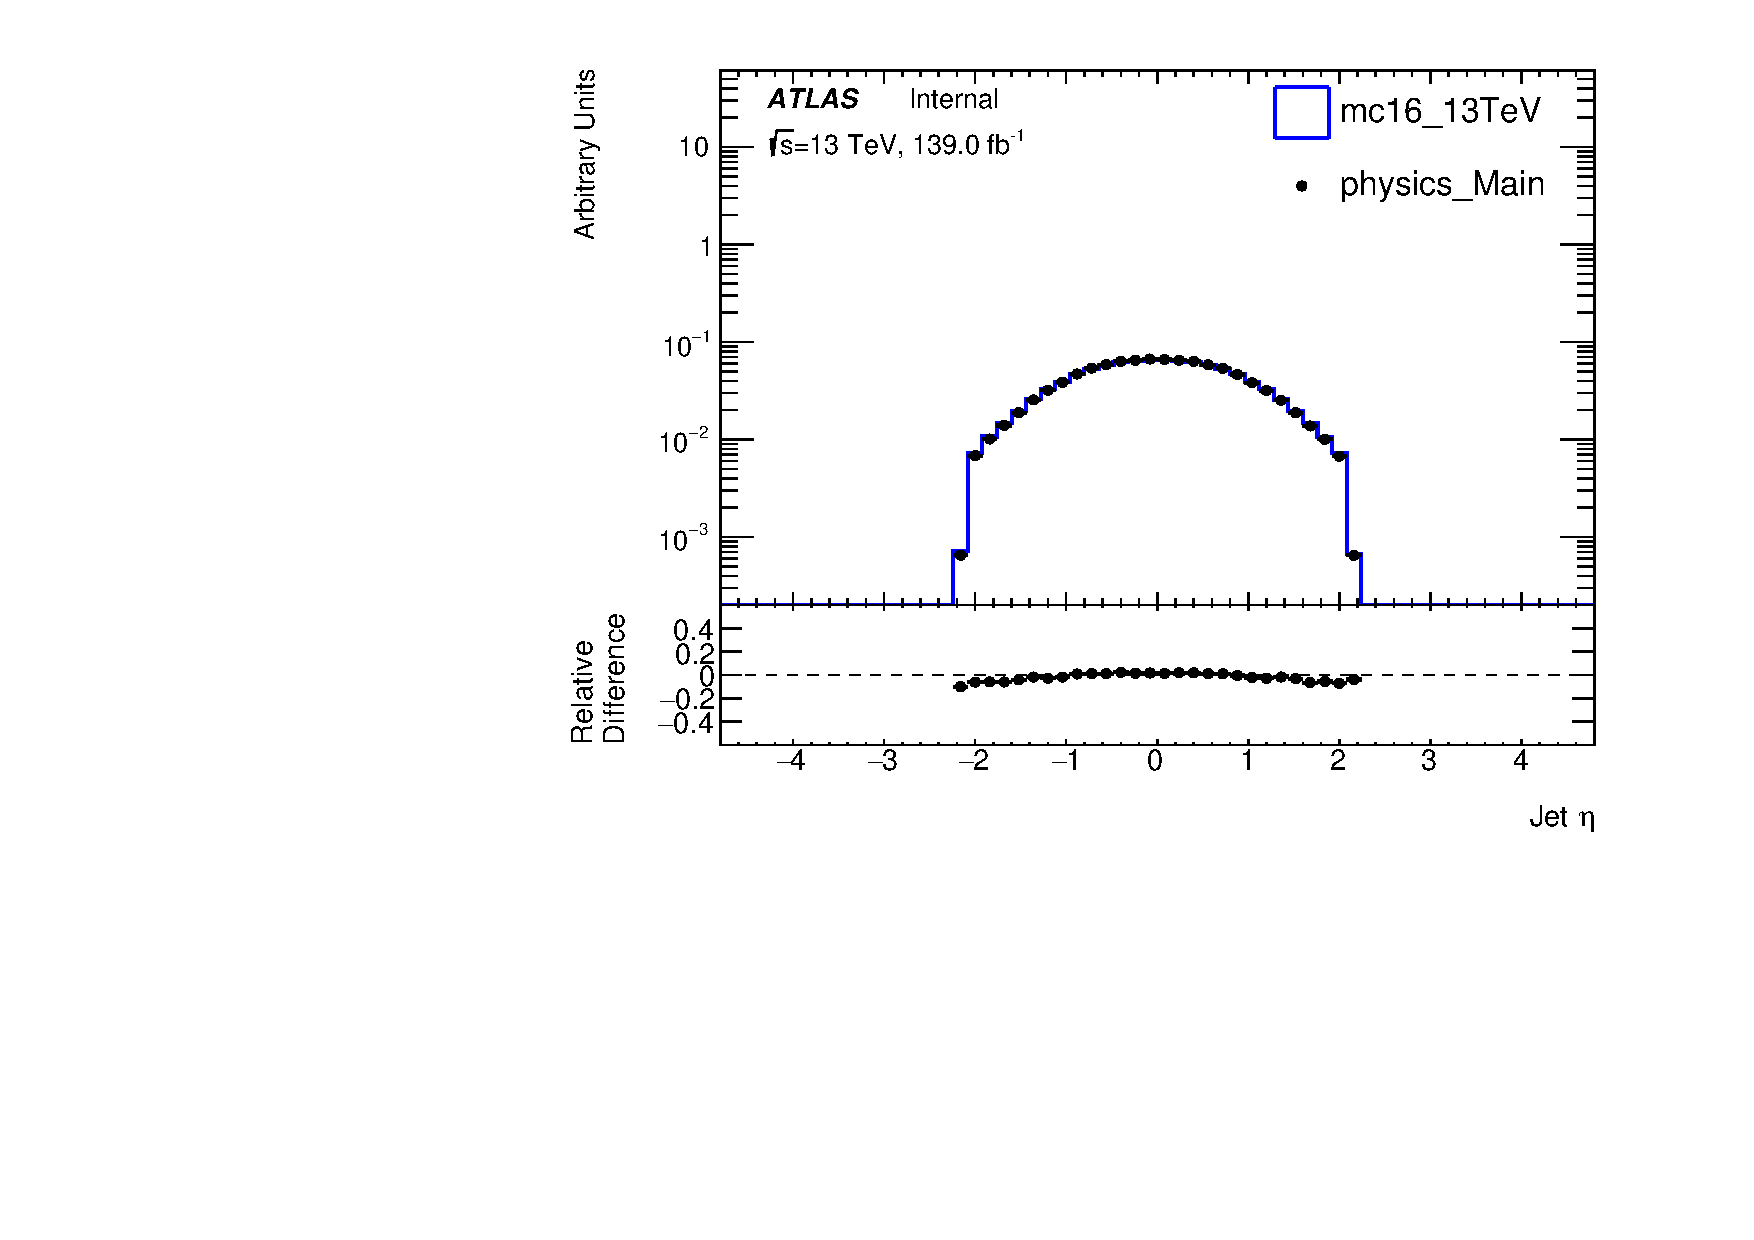
\includegraphics[width=0.45\textwidth]{figures/monitoring/GG/newStudy_jet_eta_logY_v01.pdf}}
 \subfigure[] {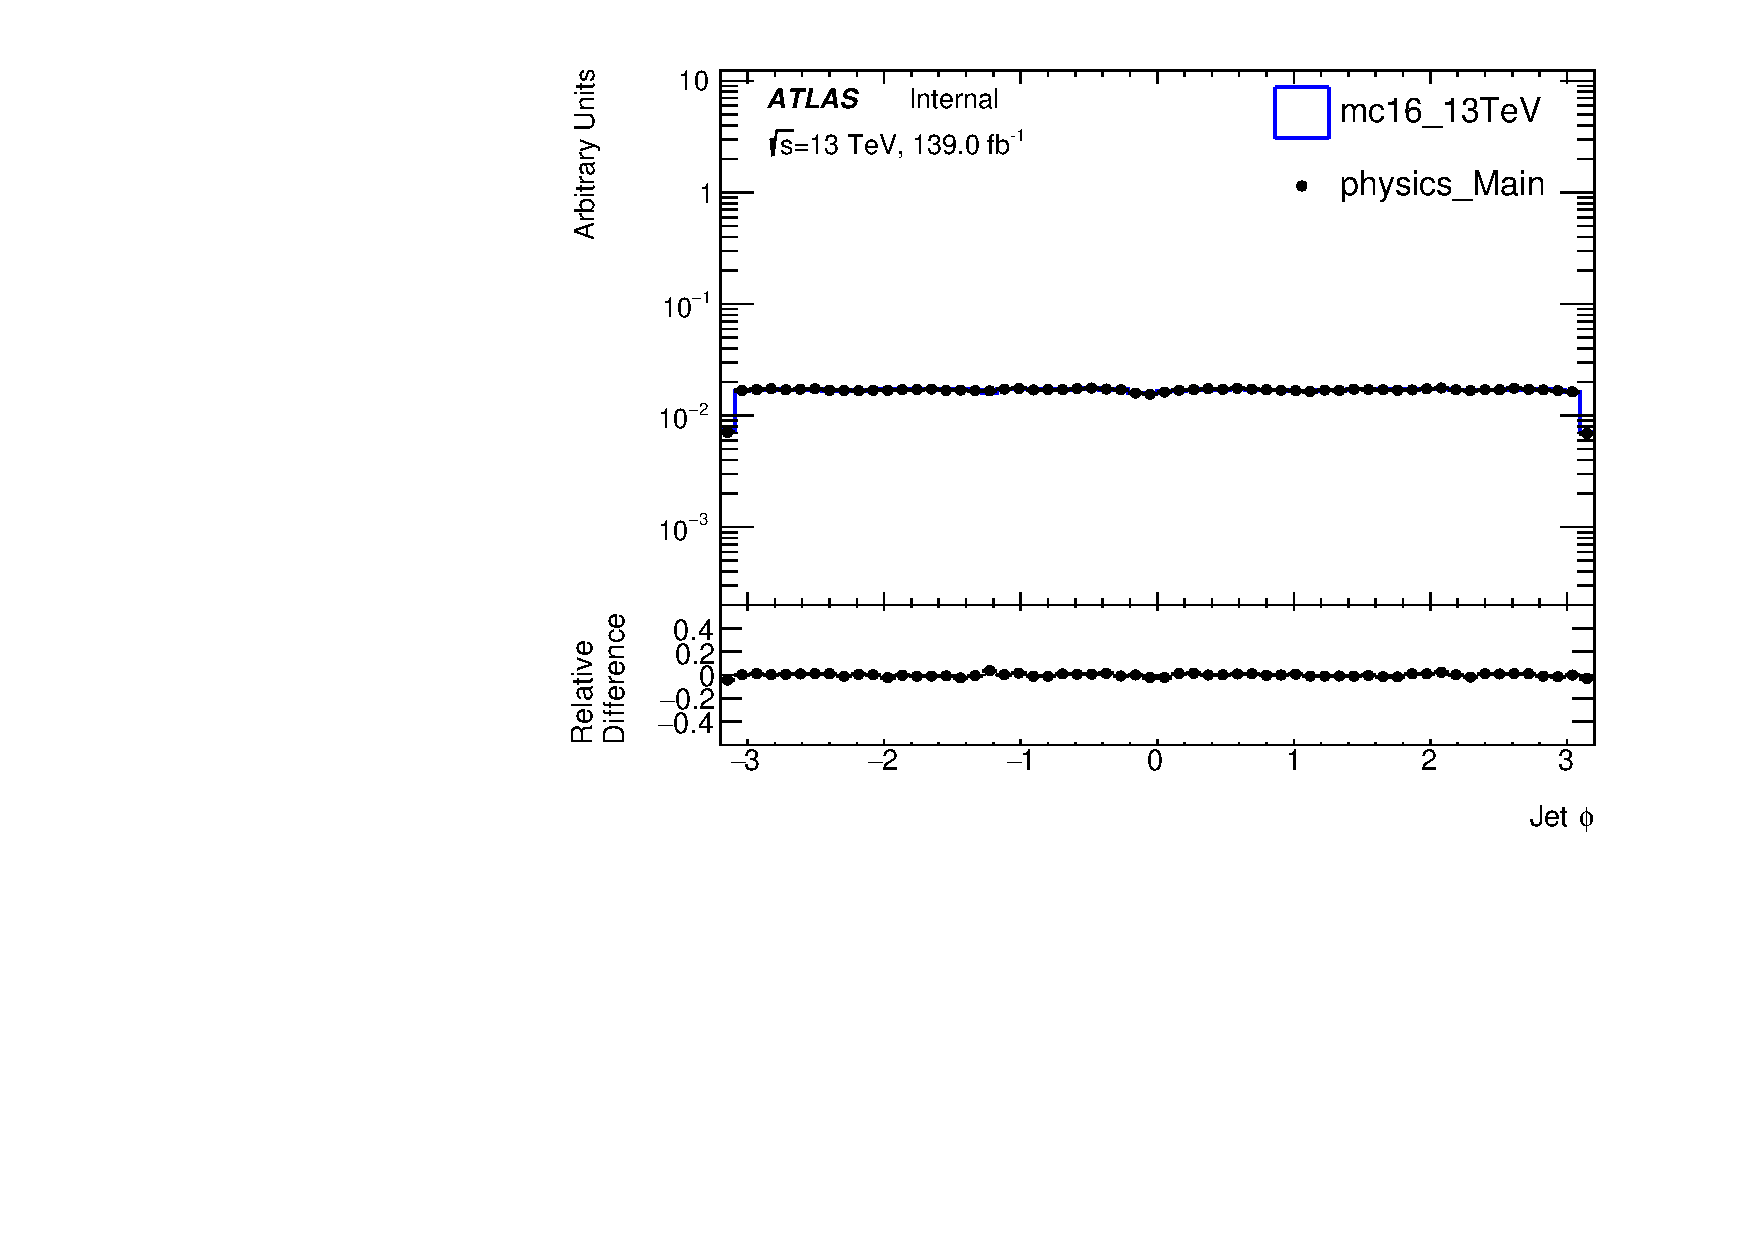
\includegraphics[width=0.45\textwidth]{figures/monitoring/GG/newStudy_jet_phi_logY_v01.pdf}}
  \subfigure[] {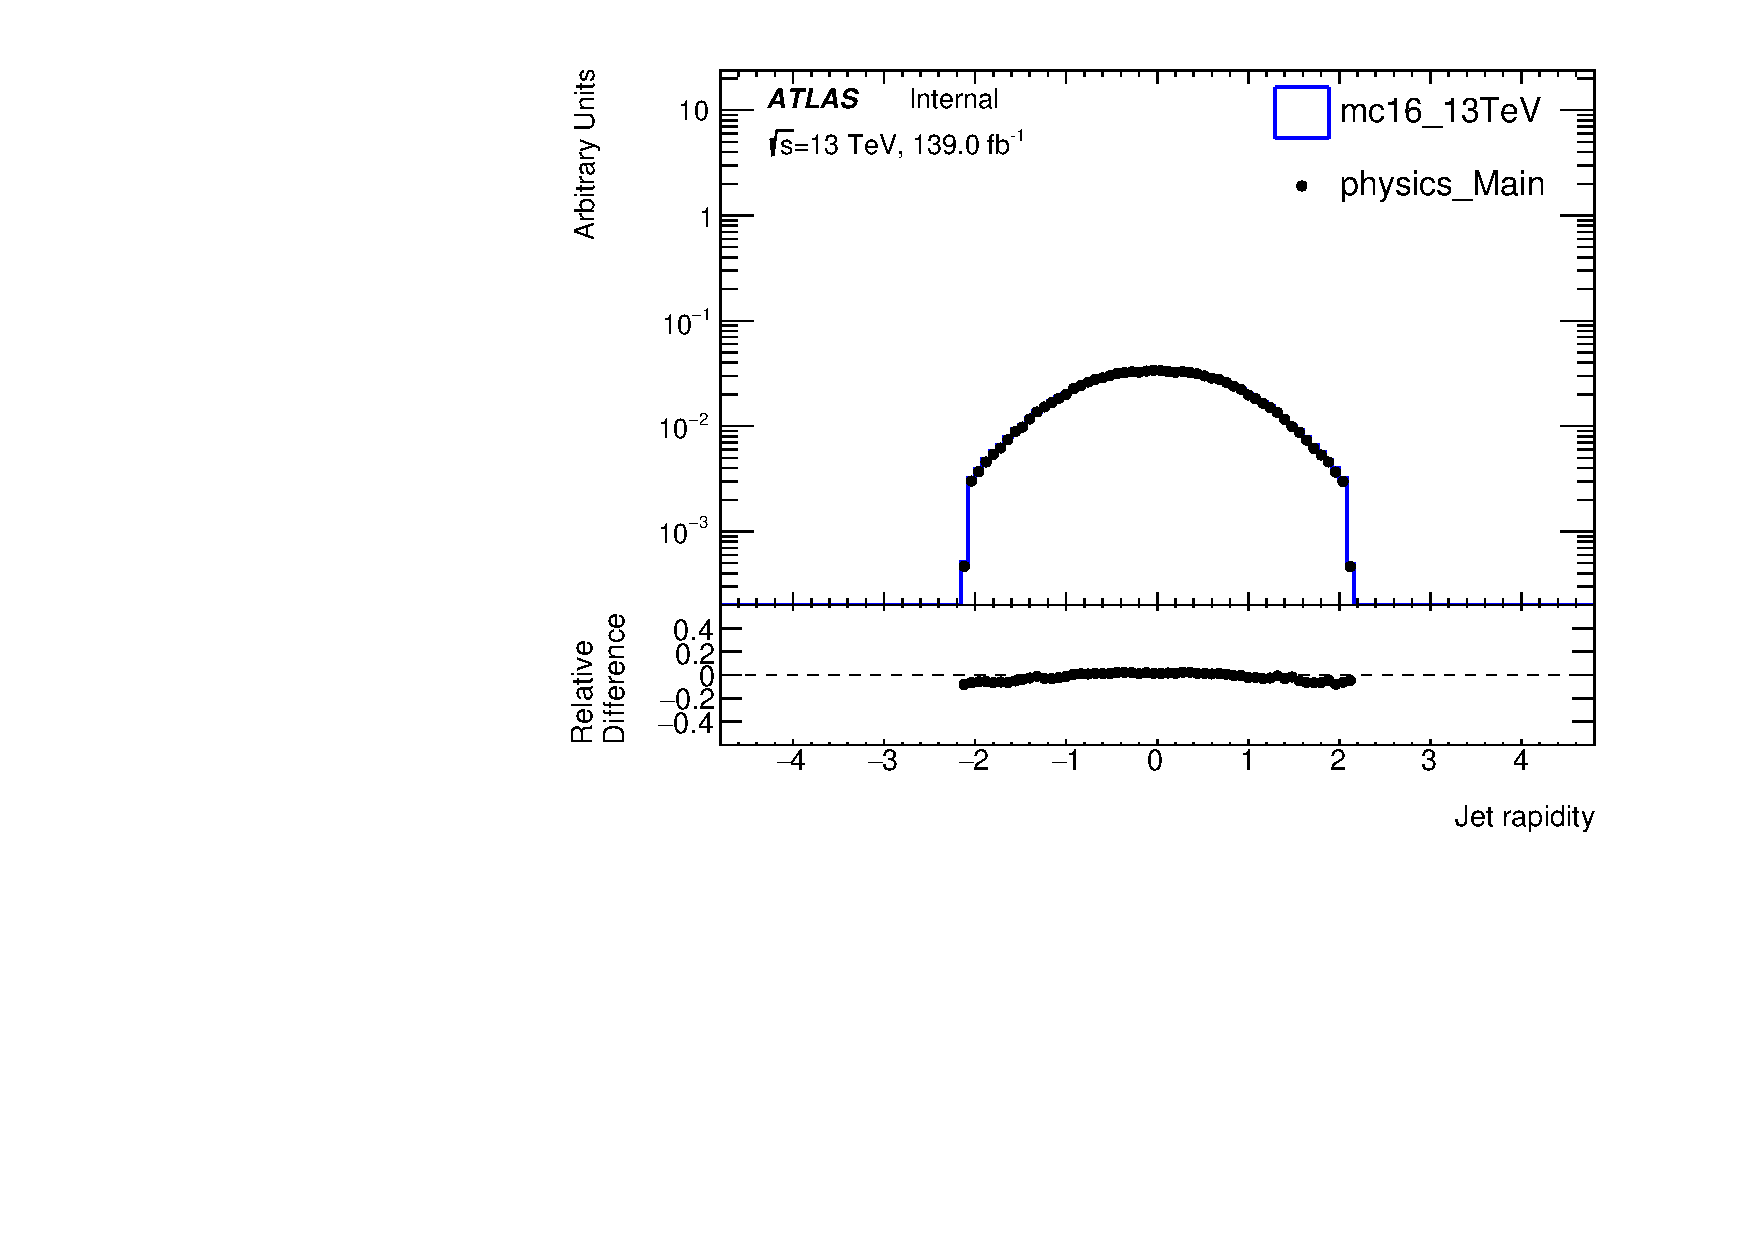
\includegraphics[width=0.45\textwidth]{figures/monitoring/GG/newStudy_jet_rapidity_logY_v01.pdf}}
 %
  \caption{Monitoring plots on  the gluon-gluon sample. 
  (a) $\Delta\phi$ between the two jets,
  (b) jet $\eta$,
  (c) jet $\phi$, and 
  (d)  jet rapidity.  %Fluctuations in the jet $phi$ distribution are attributable to dead modules in the tile calorimeter which lead to fewer jets in small slices of the detector.
  }
 \label{fig:GGmonitoring2}
\end{figure}


 \begin{figure}[htb]
 \centering
 %
 \subfigure[] {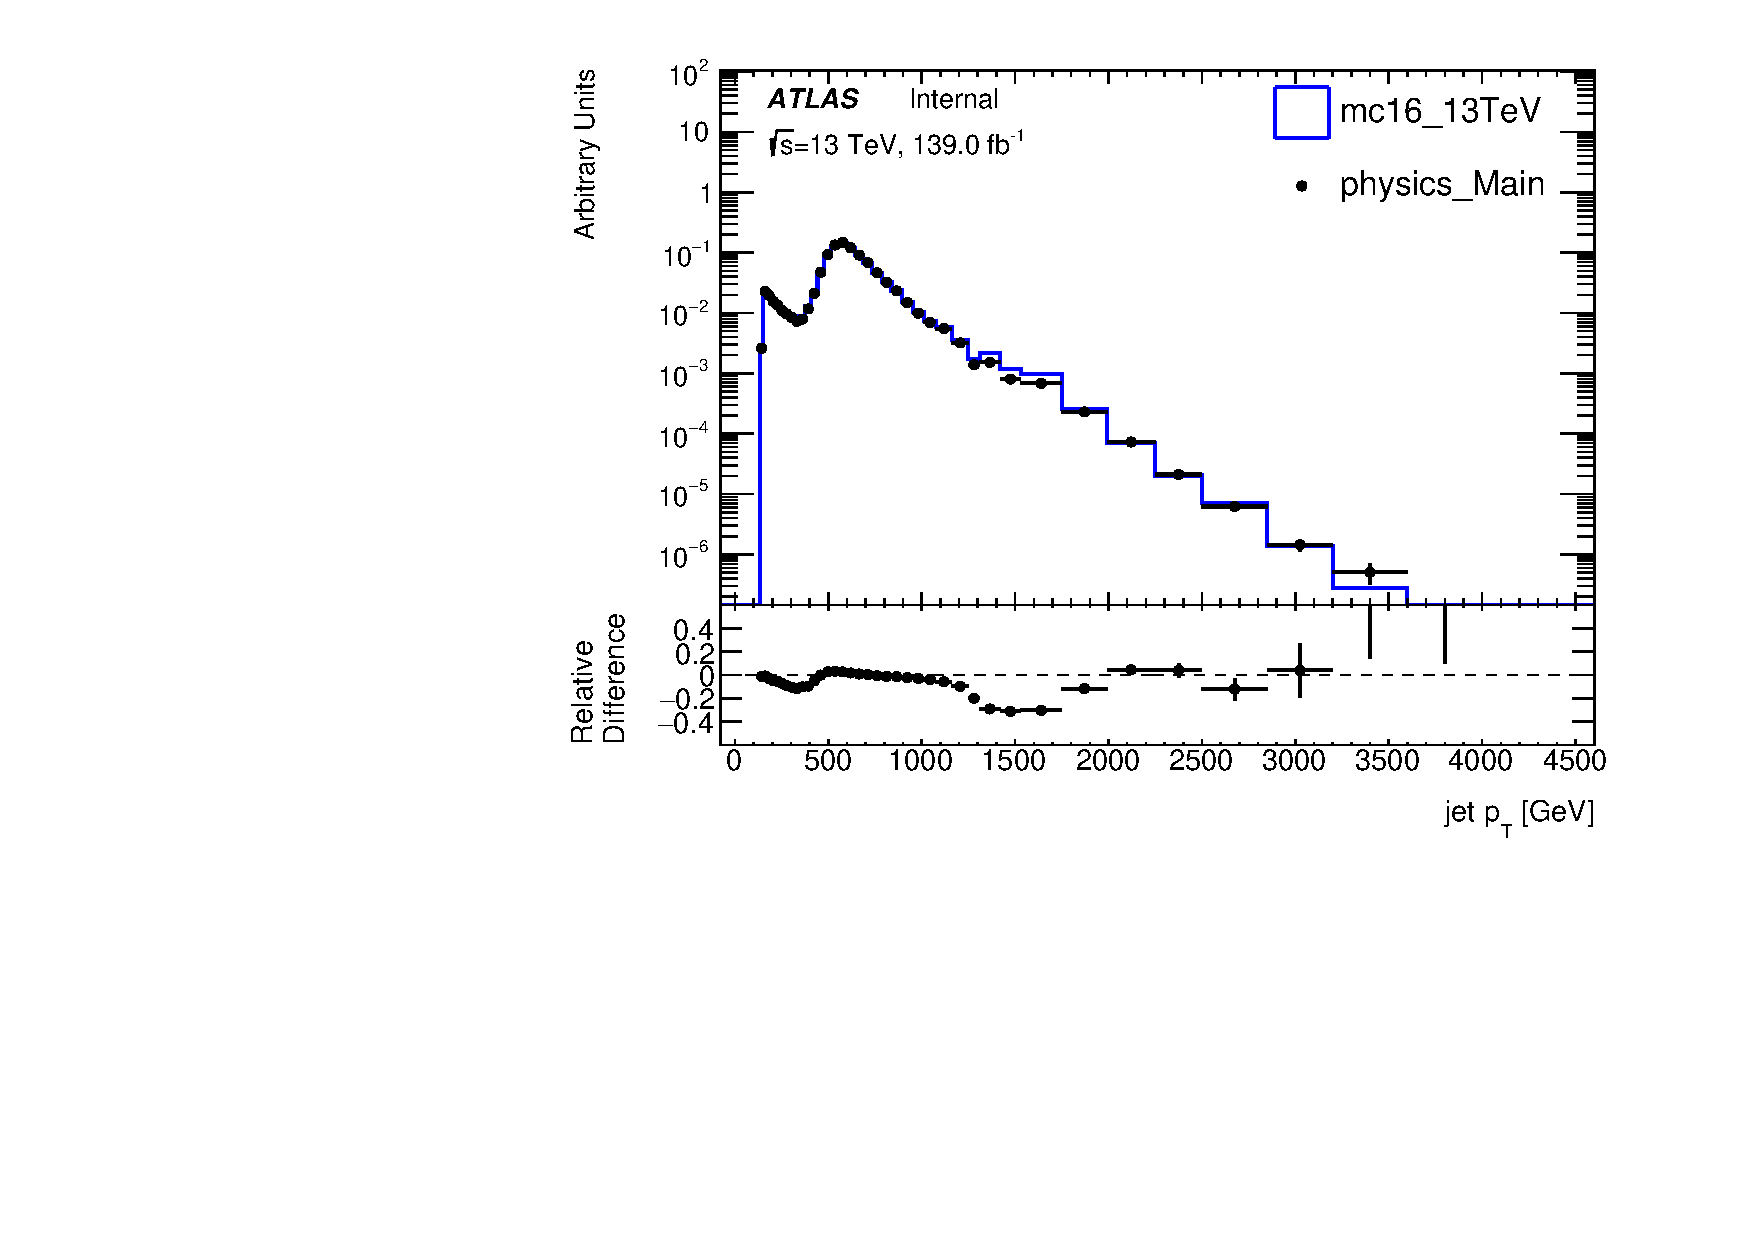
\includegraphics[width=0.45\textwidth]{figures/monitoring/GG/newStudy_jet_pt_logY_v01.pdf}}


 %
 \subfigure[] {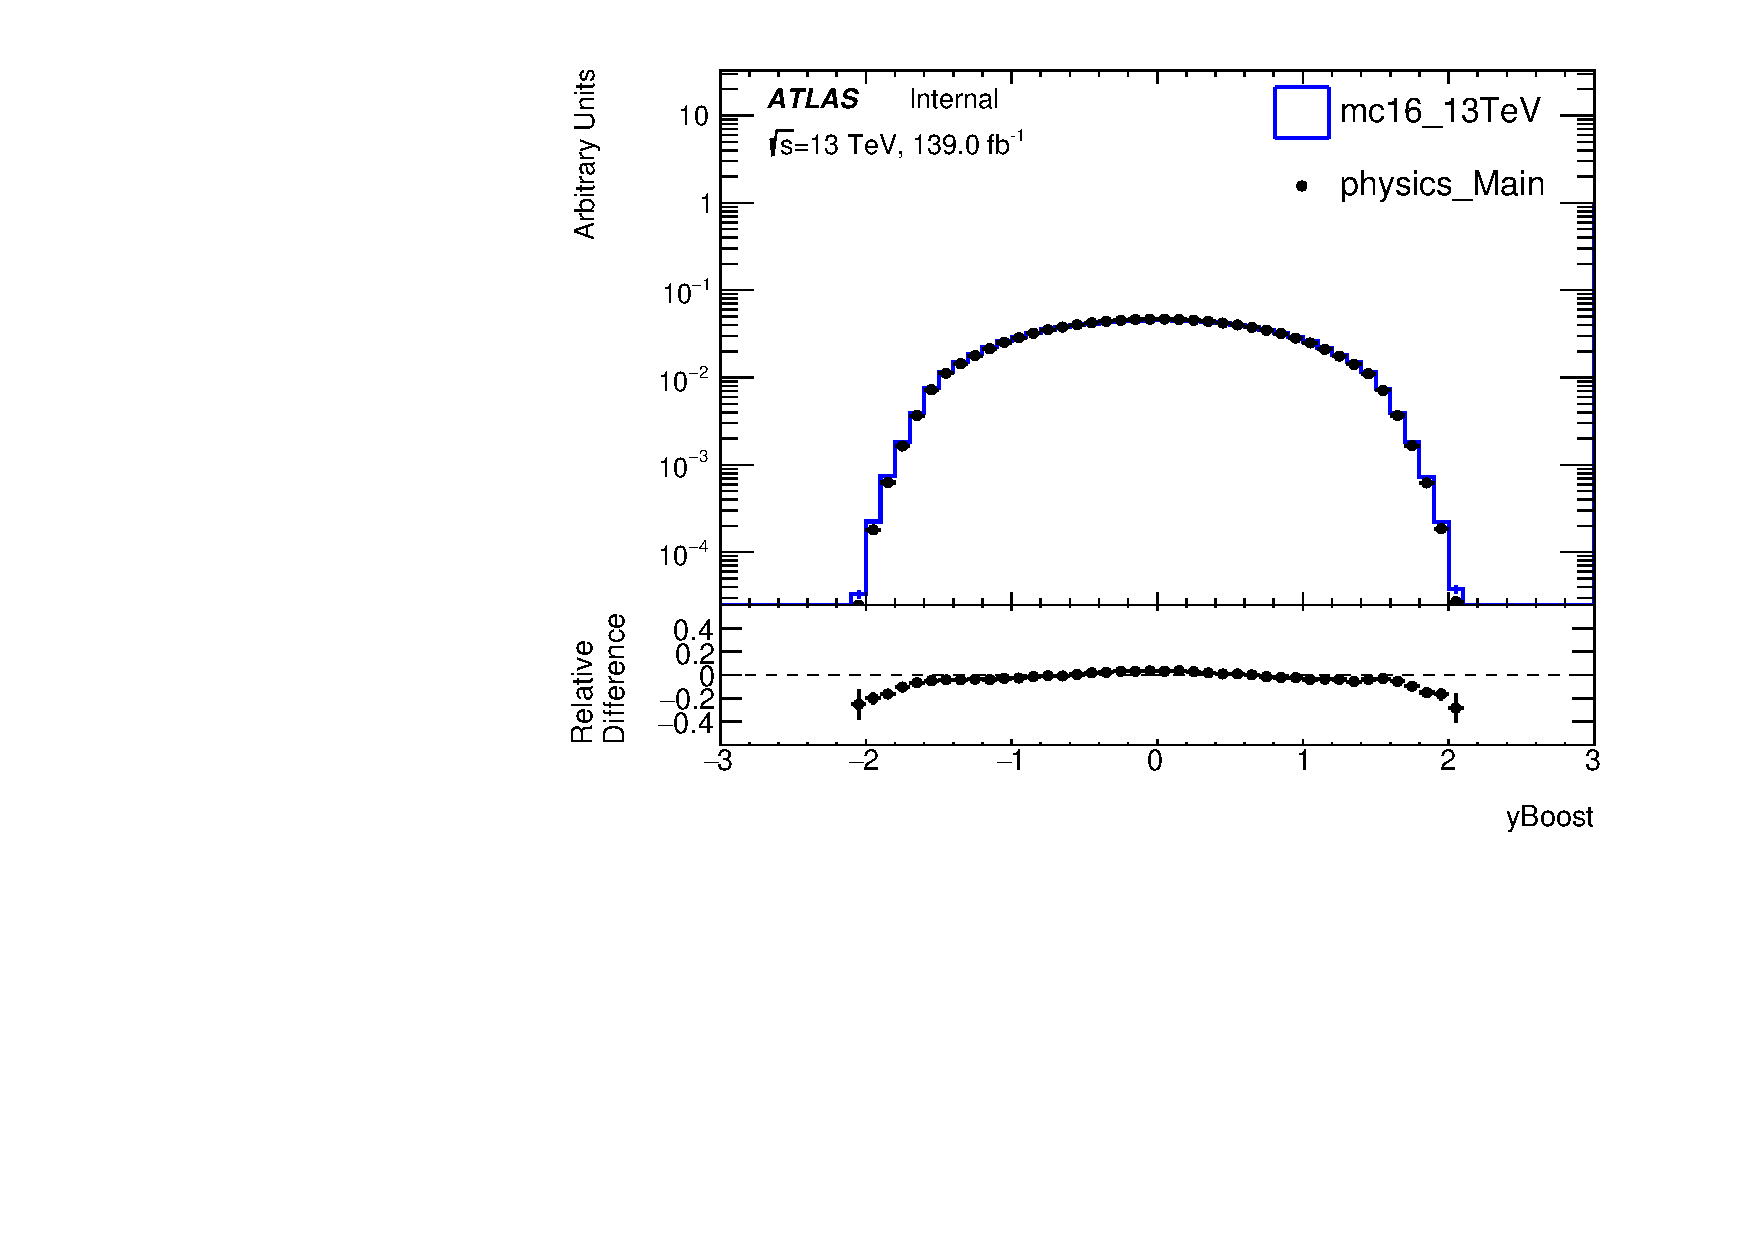
\includegraphics[width=0.45\textwidth]{figures/monitoring/GG/newStudy_yBoost_logY_v01.pdf}}
 \subfigure[] {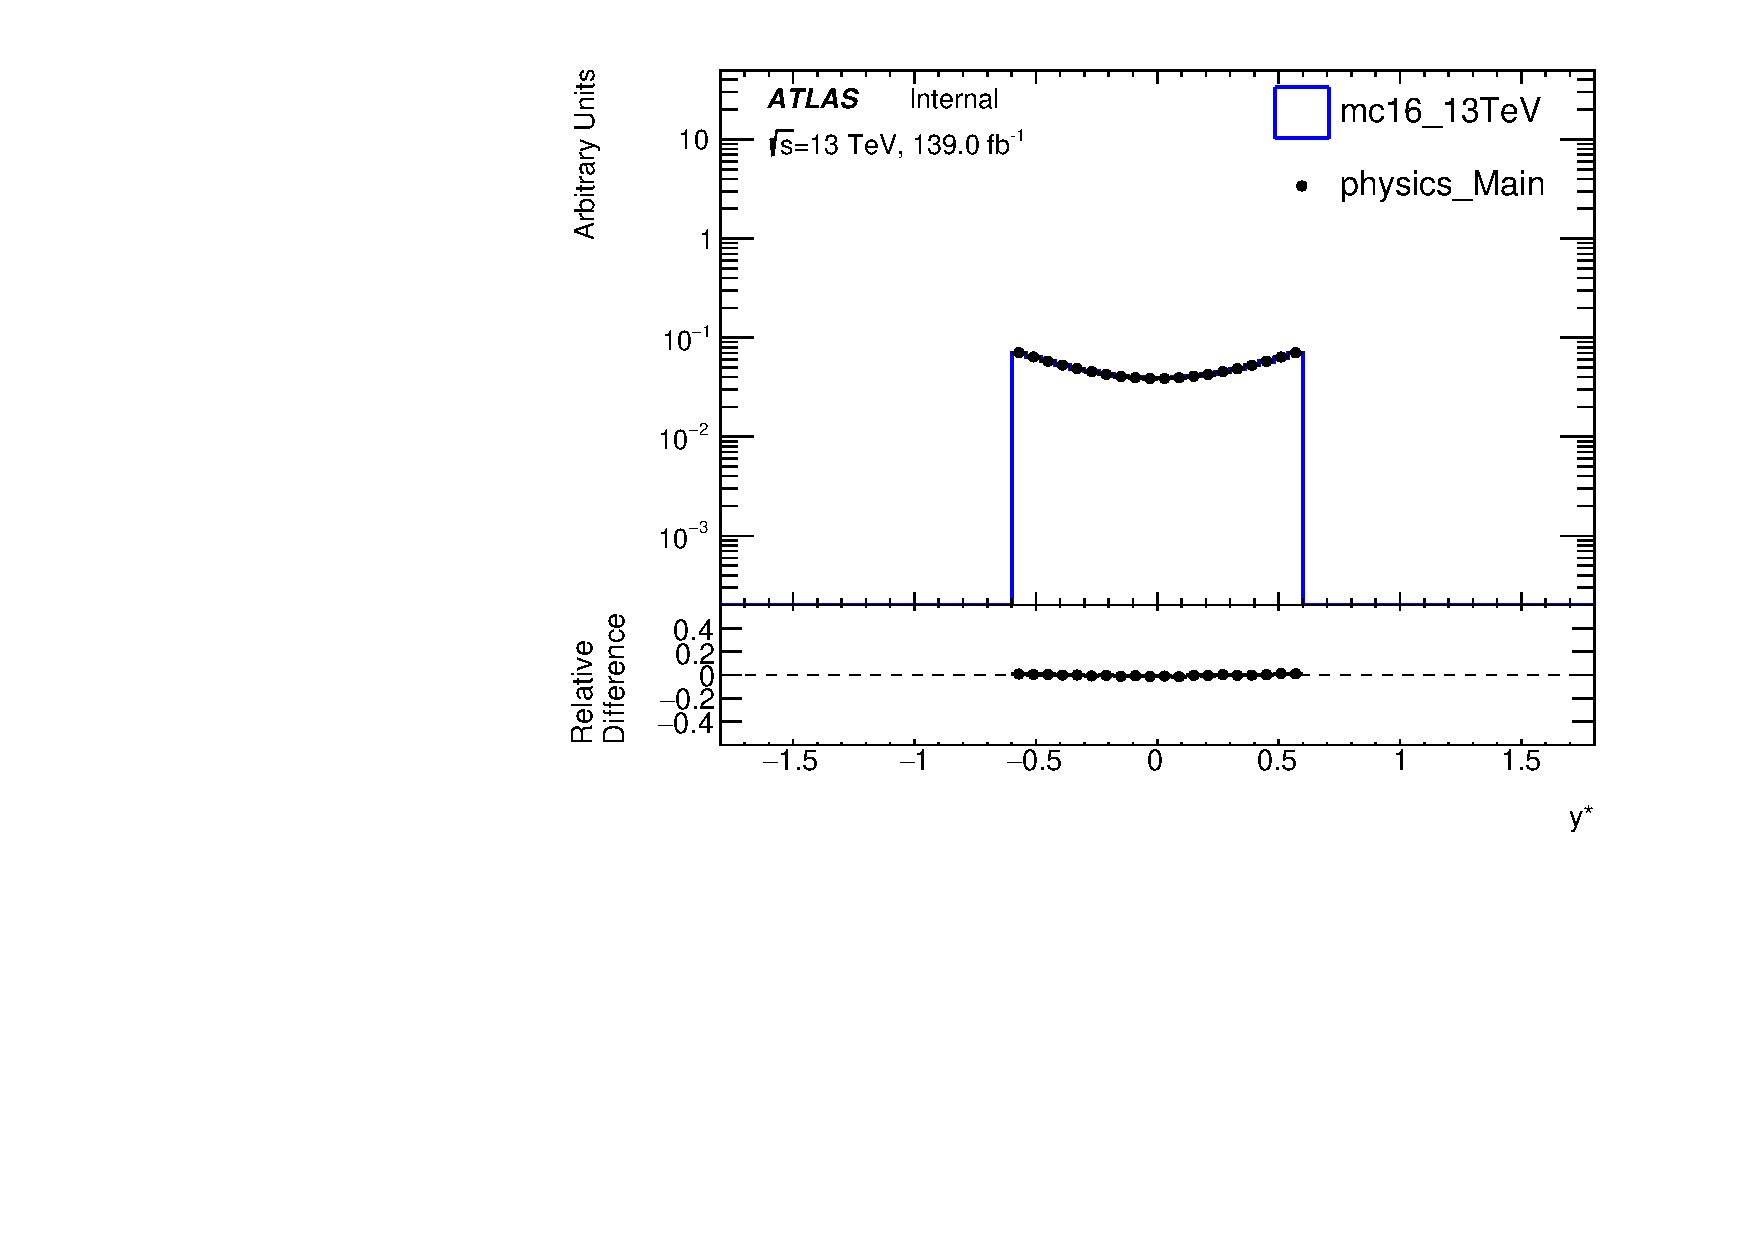
\includegraphics[width=0.45\textwidth]{figures/monitoring/GG/newStudy_yStar_logY_v01.pdf}}
 \caption{Monitoring plots on  the gluon-gluon sample.
 (a) jet \pt,
  (b) \yB{}, and
  (c) \ystar{}. }
 \label{fig:GGmonitoring3}
\end{figure}


\clearpage

